\documentclass[a4paper, 12pt]{report}

% Required packages
\usepackage{graphicx}         % For images
\usepackage{hyperref}         % For clickable links
\usepackage[english]{babel}   % Language settings
\usepackage{csquotes}         % Required by biblatex
\usepackage[left=2cm,right=2cm,top=2cm,bottom=2cm]{geometry}
\usepackage{fontspec}         % For custom fonts (XeLaTeX required)
\usepackage{tikz}             % For drawing (e.g. logo placement)
\usepackage{lipsum}           % For dummy text (optional)
\usepackage{titlesec}         % For custom chapter styles
\usepackage{float}  % Allows the [H] float placement specifier
\usepackage{listings}
\usepackage{subcaption}
\usepackage[table,xcdraw]{xcolor}
\usepackage{amsmath}
\usepackage{amsfonts} % for better fonts
\usepackage{amssymb}
\usepackage{booktabs}
\usepackage{csquotes}
% Font settings
\defaultfontfeatures{Ligatures=TeX}
% \setmainfont{Crimson}       % Optional custom font

% Bibliography
\usepackage[backend=biber,style=apa]{biblatex}

\addbibresource{mybiblio2.bib} % ✅ Make sure file name matches and is in same folder

% Chapter formatting
\titleformat{\chapter}[display]
  {\bfseries\huge\filright}{}{0pt}{\Huge}
\titlespacing*{\chapter}{0pt}{10pt}{30pt}

% Metadata
\title{new-thesis-sj}
\author{Sara Ljung}
\date{April 2025}


\lstdefinelanguage{json}{
    morestring=[b]",
    morecomment=[l]{//},
    morekeywords={true,false,null},
    sensitive=false
}

\lstset{
    language=json,
    showspaces=false,
    showstringspaces=false,
    basicstyle=\ttfamily\small,
    breaklines=true,
    frame=single,
    backgroundcolor=\color{gray!10}
}

\begin{document}
\pagenumbering{arabic}
\selectlanguage{english}

%% ------------------ TITLE PAGE ------------------
\vspace{6cm}
\begin{titlepage}
    \thispagestyle{empty} % Remove page number

    % JU logo in top-right corner
    \begin{tikzpicture}[remember picture, overlay]
        \node[anchor=north east, xshift=-2cm, yshift=-2cm] at (current page.north east) {
            
\includegraphics[width=4cm]{png/JU_A.png}
        };
    \end{tikzpicture}

    \vspace*{6cm}
    \begin{center}
        \fontsize{30pt}{38pt}\selectfont\bfseries
        Exploring AI-Based Emotion \\
        Recognition in Swedish: \\
        Speech, Text, and Vocal Markers
    \end{center}

    \vfill
    
    \textbf{Author(s):} Sara LJUNG \&{} Janna HAKKARAINEN \\  % ✅ \&{} is correct usage
    \textbf{Main subject area:} Computer Engineering \\
    \textbf{School:} School of Engineering \\
    \textbf{Date:} May 2025

\end{titlepage}

%% ------------------ BACK SIDE ------------------
\newpage
\vspace*{20cm}
\noindent
This final thesis has been carried out at the School of Engineering at J\"onk\"oping University within Computer Engineering. The authors are responsible for the presented opinions, conclusions and results.

\vspace{0.5cm}

\noindent\textbf{Examiner:} Neziha AKALIN \\
\textbf{Supervisor:} Garrit SCHAAP \\
\textbf{Scope:} 15 Credits \\
\textbf{Date:} 2025-03-09

%% ------------------ MAIN BODY ------------------
\newpage

\newpage
%%% ABSTRACT
\chapter*{Abstract}
\phantomsection
\addcontentsline{toc}{chapter}{Abstract}

\lipsum[1]

\vspace{0.6cm}
{

{\parindent=0cm\Large\textit{\textbf{Keywords:}}}
Emotion recognition, vocal markers, Swedish speech emotions, text-based emotion detection, speech-based emotion recognition 

\vspace{0.3cm}


}

\newpage

\chapter*{Acknowledgement}
\phantomsection
\addcontentsline{toc}{chapter}{Acknowledgement}

\begin{center} 
    \begin{minipage}{0.75\textwidth}
        \begin{quote}\itshape
            “The best way to predict the future is to create it.”\par
            \hfill— Alan Kay
          \end{quote}
       \begin{quote}\itshape
            “If we knew what it was we were doing, ...”\par
             \hfill— Albert Einstein
       \end{quote}
          \begin{quote}\itshape 
            "Will we go down? As far as we know,
            How do we know?"\par
            \hfill— Anna Von Hausswolff
          \end{quote}
    \end{minipage}
\end{center}
\vspace{0.5cm}

The following study is a bachelor thesis in Software Engineering at Jönköping University. As not uncommon for the female nature, behavioral 
patterns interests us, beyond doubt in combination with technology potentially holdning capacity to change not only society, but how we think. 
For the latter, it should be acknowledged, I surely hope not. 

\medskip
Thanks to Knowit, Jönköping, for supporting our project even if interdisciplinary to the general software development area. 
Thanks to our beloved computers for bringing some light into the dark night, consuming our eyes and sometimes let us forget when our brain fight. 
Thanks to all participants in this study, sharing your thoughts and a fragment of your minds, after all, it is what us all binds. 
Thanks to my thesis partner, and dear friend, Janna, you are worth more than a dime. 
Glad you read my rhyme, purhaps some joy is found when reading what is following, at least part-time. 

\medskip
Jönköping, May 2025

\medskip
Sara Ljung

\vspace{0.3cm}



\newpage

\tableofcontents

% Chapters
\chapter{Introduction}
This thesis aims to explore emotion recognition and its effectiveness in the Swedish language. With the rapid advancement of the technology industry and artificial intelligence, emotion recognition has started to play an increasingly important role in the enhancement of human-computer interactions. These areas hold potential to transform and develop several important fields, but there are still challenges in the field. Much of the research has been focused on specific languages, notably English. This research focuses on emotion recognition across two distinct modalities in Swedish, speech-based emotion recognition and text-based emotion recognition and aim to contribute to broadening the field of emotion recognition in a non-English language.

\section{Background}
Emotion recognition has attracted increasing attention with the rapid advancement of technology and artificial intelligence. Emotions are experienced by all humans but are difficult to define precisely. They are an internal experience that are foundational to our sense of identity, our relationships, and moral judgement. Scientists have faced challenges in the effort to characterize how emotions are communicated. Emotions are internal but also expressed externally through voice and movements of the body. They are not only communicated through the words we say, but also how we say them. Tones of the voice is a source of varied emotional expressions where its states may alter patterns in vocalizations. It is considered that various emotion-related physiological changes influence acoustic features such as pitch, tempo, pitch variability, and loudness in the speech \autocite{Oatley2019}.
Scientists have developed different techniques to determine states of emotions as well as opinions, a field of Natural Language Processing (NLP) that intersects artificial intelligence, computer science, and linguistics \autocite{Kansara2020}. With the development of Artificial Intelligence several techniques have accelerated in the recent years, including for NLP, even if its origins back to the 1950s when questions about whether a machine could learn and think to interact with humans \autocite{Alvarez2024}. NLP has remained as a significant contributor of AI. Some of the active research areas in the NLP domain is Machine Translation, Chatbots, recognizing speech, text summarization, and sentiment analysis \autocite{Kusal2023}. Figure \ref{fig:subdomains-AI} demonstrates the different subdomains of AI. 

\begin{figure}[ht]
    \centering
    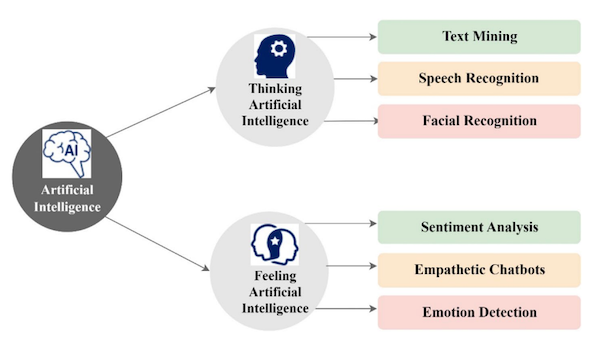
\includegraphics[height=7cm]{png/subdomains AI.png}
    \caption{\textit{Subdomains of AI \autocite{Kusal2023}}.}
    \label{fig:subdomains-AI}
\end{figure}

Sentiment analysis is a computational branch in NLP that utilizes the detection and evaluation of people’s emotions, opinions, and moods based on text, speech, facial expression, etc., without analyzing these feelings \autocite{Ermakova2023}. The rise of sentiment analysis is associated with the growth of social media, which has generated vast amounts of digital option data recorded in digital forms. Since the early 2000’s, the field has become one of the most researched parts in NLP \autocite{Zhang2018}, expanding beyond computer science to fields like finance, marketing, political- and health science. Accordingly, sentiment analysis is valuable across different areas of society. Sentiment analysis is utilized in the popular index called the happy planet index \autocite{HappyPlanetIndex}, measuring sustainable well-being of different countries, even if it only can observe three feelings, positive, negative, or neutral. The happy planet index checks the happiness level calculated from a particular country, where emotion detection is used with sentiment analysis \autocite{Madhuri2021}.
With the evolution of deep learning networks, emotion detection has advanced. Sentiment analysis identifying positive, negative, or neutral states have progressed into recognizing the six basic emotions; joy, sadness, anger, disgust, fear, and surprise in text \autocite{Safari2023}. The emotions categorization fluctuate depending on the research. These basic six where determined by Paul Ekman \autocite{Oatley2019, Kusal2023} who determined that these six fundamental emotions is shared in people of different cultures, characterized by facial features. However, Ekman’s classification was made over 20 years ago when no agreement about what emotions should be considered as existed. Today, the agreement about evidence for universal emotional signals and evidence for five emotions is robust: anger, disgust, sadness, happiness, and fear \autocite{Ekman2016}.

Emotion recognition is accomplished either through text or speech, with numerous studies in both areas. Text-based emotion detection is a complex field that requires a very clear understanding of the context. Today this technique is frequent in several fields, such as human-computer interaction, big data, data mining, e-commerce, online tutorials and psychology \autocite{Madhuri2021}. The first emotion dataset, The International Survey on Emotion Antecedents and Reactions (ISEAR) was developed in 1997, after it was stated that computers need the ability to interpret, express, and identify emotions if we want true intelligent computers and be able to communicate with them naturally \autocite{Kusal2023}.

Emotion recognition from textual data is important in various domains such as customer reviews, social media analysis, public monitoring, and conversational agents. A systematic review \autocite{Kusal2023} shows that Deep Learning models outperform traditional Machine Learning models due to their ability to capture contextual dependencies. The review further demonstrates the highest accuracy is shown by transformer-based models such as bidirectional encoder representations from transformers (BERT), highlights challenges such as small or imbalanced datasets that can affect the model reliability, and notes that multimodal approaches with text, speech, and images improve emotion recognition. BERT-technology is leveraged with a model that outperformed other text-based emotion recognition models, with 76\% validation accuracy \autocite{Madhuri2021}. However, text-based emotion detection (TBED) has challenges with identifying hidden emotions, and adapting to diverse languages. Datasets based on different languages than English, as Arabic and Hindi, are tested in a study \autocite{Maruf2024} that identifies challenges as limited resources for non-English languages. The authors underscore the potential of TBED but notes limitations as it is no universal solution for challenges like sarcasm, dynamic emotions, and cultural variances.

Emotion detection research progressed with Speech Emotion Recognition (SER) \autocite{Kusal2023}. It has shown that hearers can evaluate five emotions in speech-prosody, anger, happiness, sadness, fear, and tenderness, with 70 percent accuracy \autocite{Oatley2019}. Speech emotion recognition focuses on how something is said rather than the words themselves. Acoustic features like amplitude, formants, and pitch help classify emotions. A common approach uses Mel-frequency cepstral coefficients (MFCCs), which capture vocal patterns and have proven effective in detecting emotions \autocite{Thaler2024}. Those features offer invaluable insights into the subtle emotional expressions conveyed through speech, assisting the complicated process of emotion recognition. They are typically categorized into three primary groups: prosodic features, voice quality features, and spectral features \autocite{Lian2023}.

Several studies distinguish different emotions through vocal features. Already in 2005, Lee \& Narayanan investigated automatic recognition of emotions, especially positive vs. negative from spoken dialogs. In that study, acoustic, lexical, and discourse information were combined to enhance emotion detection and move beyond traditional acoustic-only ways. The authors analyzed acoustic features, lexical features, and discourse features. Linear Discriminant Classifiers were used and resulted in good performance for acoustic and lexical information \autocite{ChulMinLee2005}. In 2014, one study \autocite{Bnziger2014} showed that regular people can rate how voices sound reliably, when actors pretend to feel emotions, sometimes better than machine sound measurements for pitch and volume. The human voice feature rating worked better than technical measures, especially for happy emotions. 
These acoustic features in our voice enable emotion recognition through speech using Deep Learning, which have many advantages for Speech Emotion Recognition over traditional sentiment methods. Deep Learning has the capability to detect complex structures and different features without requiring manual feature extraction \autocite{Khalil2019}. SER’s goal is identification of emotions in speech, unrelated to the semantic content \autocite{Kusal2024}. Figure \ref{fig:blockdiagram-SER} represents a SER system. 

\begin{figure}[ht]
    \centering
    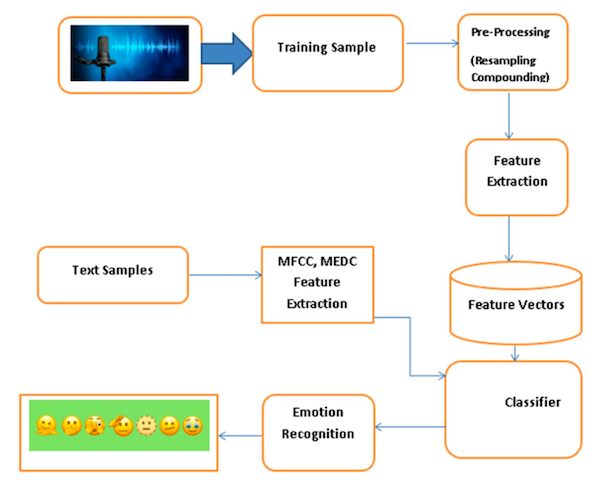
\includegraphics[height=7cm]{png/blockDiagram SER.png}
    \caption{\textit{Block diagram of SER \autocite{Tyagi2024}.}}
    \label{fig:blockdiagram-SER}
\end{figure}

In recent years, speech emotion recognition has emerged as a significant and complex research area within pattern recognition, speech signal processing, and artificial intelligence. Its growing importance is driven by its applications in human-computer interaction. Specifically, SER systems enable emotion-aware interactions through speech, eliminating the need for traditional input devices. This advancement has led to the development of intelligent affective services in fields such as call centers, healthcare, surveillance, and affective computing \autocite{Zhang2021}. The accuracy of models tested in recent years have improved significantly. Several studies conducted in the last year’s show emotion detection accuracy results over 90\% \autocite{Adebiyi2024, Praseetha2022, Rahman2024}. A research paper \autocite{Abbaschian2021} compares several studies, detailing the results, databases used, and the time periods during which the studies were conducted. The reported accuracies depends greatly on which model was used, as well as the tested dataset. According to Abbaschian (2021), in 2014, one model showed 54.3\% accuracy for the IEMOCAP dataset. The same dataset was used for the LSTM model in 2017 and 2018 with 63.5\% respectively 64.93\% accuracy. When the same dataset was tested with a CNN-model, the accuracy increased to 82.8\% in 2019.  

A study \autocite{Juslin2018} concluded in 2018 analyzed 1,877 voice clips from 23 datasets to compare spontaneous and posed emotions. Their findings highlighted key differences: 
\begin{itemize}
    \item Spontaneous expressions were rated as more genuine than posed ones, even when intensity was controlled. 
    \item Posed expressions were more intense, but intensity alone did not fully explain perceived authenticity. 
    \item Acoustic differences were small but present, mainly in pitch range, speech rate, and voice intensity. 
    \item Highly intense spontaneous emotions conveyed emotions as clearly as posed ones, suggesting that emotion intensity plays a role in perception. 
\end{itemize}
These findings suggest that posed and spontaneous emotions are not interchangeable and that datasets used in SER research must account for these differences to ensure reliable models. 

One study \autocite{Rathi2024} presents a comprehensive review of SER which explores the impact of speech data corpora selection and speech feature extraction on the accuracy of emotion classification. Publicly available speech datasets from 2014-2023 are systematically analyzed and categorize speech datasets and speech features to evaluate their impact on the accuracy of emotion recognition. The study by Rathi \& Tripathy (2024) includes the six emotions: happiness, anger, sadness, surprise, fear, and neutrality. According to Scherer, Frühholz \& Belin (2018), most studies focus on only four broad emotion categories: anger, fear, happiness, and sadness, which is seen as a limitation by the authors \autocite{Scherer2018}. However, emotion classification fluctuates in different studies. A database has been conducted that unravel this limitation. The database is called GoEmotions \autocite{Demszky2020} which is a big, detailed, and reliable dataset for recognizing 27 emotions in text. The researchers \autocite{Demszky2020} used a BERT model and got an average F1-score of 0.46 for these emotions, best for gratitude (0.86) and worst for grief (0.00). The model performed a score of 0.64 for the simpler 6 emotion grouping. The authors conclude that the model still needs advancements for tricky feelings but suggest the model as a good starting point. This research is included in the research that the AI-model Hume.ai builds upon \autocite{HumeAI-AboutHume}, which is important to acknowledge since it might affect biases. Most researchers focus on the fundamental and widely recognized emotions. The six fundamental emotion model by Paul Ekman is the most widely used for both text-based and speech-based emotion recognition \autocite{Maruf2024}.

Datasets are essential for data-driven learning, enhancing model performance and robustness. Emotion recognition datasets are classified based on signal type, including speech (textual/audio), visual, physiological signals, and multimodal data. Speech emotion datasets are further classified by how they are collected: 
\begin{itemize}
    \item Performer-based datasets feature emotions acted by trained performers. 
    \item Induced datasets capture emotions in controlled environments, making them less expressive but closer to real-life emotions. 
    \item Natural datasets come from real conversations (e.g., public dialogues, call centers) and contain authentic emotional variations but are more challenging due to background noise and limited availability \autocite{Cai2023}. 
\end{itemize}
Most research in the field of SER investigates the accuracy of different Deep Learning algorithms on diverse public datasets. A review \autocite{Rathi2024} analyses 93 research papers where IEMOCAP and RAVDESS are among the most widely used datasets, chosen by 35.83\% and 21.50\% of researchers, respectively. Their popularity stems from well-annotated data and diverse range of emotional expressions, which enhance model performance. Figure \ref{fig:datasets-percentage} presents the usage of the datasets in this review.  
\begin{figure}[ht]
    \centering
    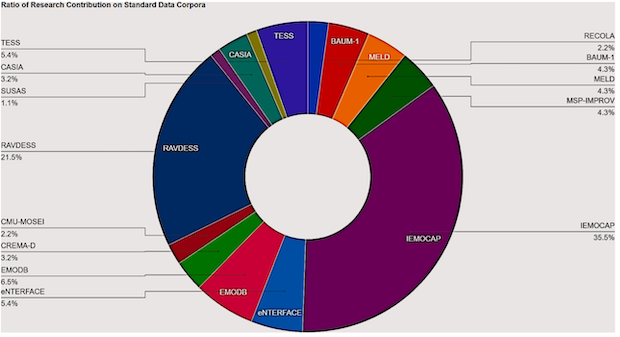
\includegraphics[height=8cm]{png/datasets percentage.png}
    \caption{\textit{Research contributions of standard data corpora in percentage}\autocite{Rathi2024}.}
    \label{fig:datasets-percentage}
\end{figure}
The paper \autocite{Rathi2024} includes varying datasets in terms of linguistic diversity, recording conditions (acted, induced, or natural speech), and the number of emotional categories. The results show that the choice of dataset significantly affects the model's performance. Key features such as Mel-Frequency Cepstral Coefficients (MFCCs), pitch, intensity, prosodic cues, and spectral properties impact SER accuracy significantly. The authors discuss the balance between realistic datasets and classification accuracy, noting that natural speech is more difficult to classify due to its high variability and noise in natural speech. 

The number of natural datasets is relatively limited \autocite{Cai2023}, and many research papers test on acted datasets. An empirical analysis \autocite{Ahammed2024} of Machine Learning algorithms across diverse datasets, concluded in 2024, demonstrates high-accuracy SER system using an SVM classifier and advanced feature extraction techniques. The model performed exceptionally well across multiple datasets (RAVDESS, TESS, SAVEEE, and combined dataset), with the combined dataset achieving perfect scores (100\%) in accuracy, precision, and F1-score. Two of these datasets, RAVDESS \autocite{StevenRLivingstone2019} and TESS \autocite{Pichora-Fuller2020}, are acted and the SAVEE \autocite{kaggle-savee} dataset was recorded from four male, postgraduate students and researchers. All three datasets are in recorded in English. 
The TESS dataset was used in a study from 2022 \autocite{Praseetha2022} that leveraged other techniques, with one original dataset and one augmented dataset. Achieved accuracy was 93\% and 97\% for the augmented dataset, resulting in a significant improvement for the processed data.
A different study \autocite{Alroobaea2024} from 2024 investigates transformers for SER in cross-corpus scenarios. The recordings are preprocessed to remove noise, and augmented techniques are applied. Three datasets were used, two the same as the previous study, SAVEE and RAVDESS, with the Berlin Database of Emotional Speech, Berlin EMO-DB, including ten professional speakers, was additional. A combined cross-corpus dataset of the three sets were used to test generalizability across different datasets. This proposed transformer-based model outperformed traditional deep learning methods. The model showed high accuracy results with 95\% for SAVEE, 94\% for RAVDESS, 97\% for EMO-DB, and 97\% for the cross-corpus dataset. However, this model was not evaluated on spontaneous speech datasets.
Comparing these three studies from 2022 to 2024 reveals a clear trend of increasing accuracy over time. A 2019 review \autocite{Khalil2019} reported significantly lower results for the SVM, with accuracy of 74\% for anger, 70\% for happiness, and 93\% for sadness. However, the same study found that a Deep Convolutional neural network (DCNN), achieved substantially higher accuracy, with 99\% for both anger and happiness, and 96\% for sadness. Both Emo-DB and SAVEE datasets were included, as well as IEMOCAP which also is an acted dataset recorded in English.

Datasets for Text Based Emotion Detection (TBED) are discussed in \autocite{Kusal2023}, where the authors state that researchers can use publicly available datasets or create their own. Publicly available, useful datasets with reliable annotating include several sets based on various data, from stories, publications, news, social media texts, to reviews on movies. The datasets emotion-classification reaches from the basic six emotions to GoEmotions set that include 27 emotions. Many datasets are based on social media, including casual writing style which is a big challenge. The use of short messages and informal language has limited research. Human emotion expressions and the texts conveying them are ambiguous and subjective, additionally, emotions are multifaceted with varying expressions. Therefore, the authors claim that human mapping is important. 
Self-labeled emotion datasets are tested in a study \autocite{Lee2023} that uses a Transformer Transfer Learning (TTL) model trained on a dataset of over 3.5 million tweets with self-reported emotion hashtags. The model is tested against 10 prior published datasets and achieved highest score on annotator-rated sets (0.87), it also performed well on self-reported sets (0.79) which demonstrates generalizability.  

The promising development of emotion recognition has been adapted in research for other areas than computer and machine learning science. SER is beneficial in translating languages, interactive courses and tutorials held online where the student’s emotional state can be understood to help the machine make decisions on how to present the course. It can be implemented in vehicles’ safety structures to recognize the driver’s emotional state and therefore prevent accidents \autocite{Abbaschian2021}. The mental health sector has great potential to benefit from emotion recognition. Several studies \autocite{DeSouza2021, Drougkas2024, Simcock2020,Singh2023} have investigated how AI-based emotion recognition can be used to help therapists and psychiatrics diagnosing and identifying potential mental illnesses. One of the studies \autocite{DeSouza2021} demonstrates how leveraging speech and text analysis with NLP can help detect late-life depression. It showed consistent alterations in individuals with depression, including acoustic features such as pitch, speech rate, pause duration, and word choice. The authors suggest that automated speech analysis can identify late-life depression as well as predicting depression severity with accuracy of 86-92\%. Multimodal machine learning with a combination of text and audio analysis has been explored to identify indicators for various mental health disorders. The research \autocite{Drougkas2024} compared unimodal text models, which showed strong results but was outperformed by the multimodal models, especially for identification of the presence of markers. The multimodal models achieved accuracy up to 86.73\%. This study highlights the importance of machine learning integration in mental health diagnostics. 

\section{Problem Description}
Despite significant progress in speech emotion recognition, there are limitations in current research. For instance, emotional voice samples are usually obtained from actors portraying emotions using scripted speech. These acted expressions tend to be more intense and exaggerated than naturally occurring emotions. However, this method risks overemphasizing obvious emotional cues while missing subtle ones. It is argued that such portrayals reflect social norms more than genuine physiological responses, although all public expressions may involve some degree of performance \autocite{Scherer2018}.

The way emotional speech data is collected depends on the design and purpose of the SER system. As datasets shift from acted emotions to more spontaneous or real-life emotions, emotion recognition becomes more challenging. Many researchers prefer acted emotion datasets because they offer a wide range of emotions and large amounts of data \autocite{Rathi2024}. Induced datasets are collected by constructing an artificial emotional situation, without the knowledge of the performer or speaker. This results in a more naturalistic database, but issues regarding ethics may apply, since the speaker should know they have been recorded for research \autocite{Khalil2019}. 

Estimation of emotions from spontaneous speech is a challenging task. Most studies test models on acted datasets \autocite{Khalil2019, Ahammed2024, Praseetha2022, Alroobaea2024}. The primary reason for the concentration on acted SER tasks is that acted emotions can be easily performed in a controlled laboratory setting, often resulting in high SER accuracy. However, these emotions tend to be exaggerated and may not accurately reflect how emotions are expressed in real-world situations. Consequently, detecting spontaneous emotions in natural environments is significantly more complex and challenging compared to recognizing acted emotions \autocite{Zhang2021}. Figure \ref{fig:databases-diff} demonstrates the difficulty level for varying settings.

\begin{figure}[ht]
    \centering
    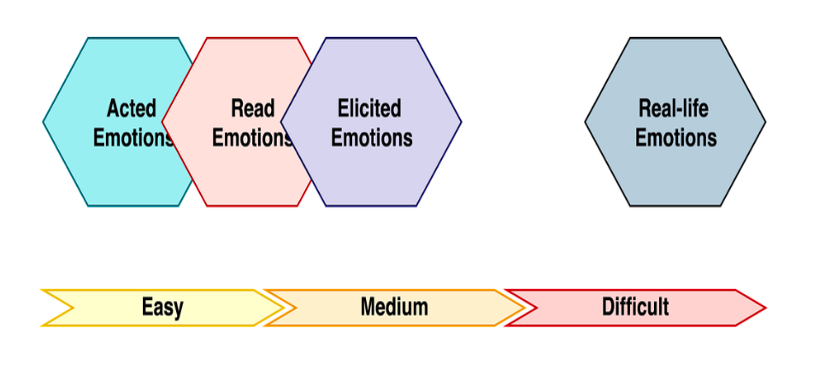
\includegraphics[height=6cm]{png/databases difficulty.png}
    \caption{\textit{Emotion recognition databases and their difficulty level \autocite{Khalil2019}.}}
    \label{fig:databases-diff}
\end{figure}
One study from 2019 \autocite{Milner2019} using four English speech datasets, two acted (eNTERFACE and RAVEDESS), one elicited (IEMOCAP), and one natural (MOSEI), to see how emotions can be recognized across them. The researchers in this study tested different training methods to explore whether mixing acted and natural data works. They found that acted data does not easily help with natural emotions unless the system is tweaked. The differences in real and acted voices are shown in other studies as well \autocite{Juslin2018}. Real ones sound more genuine and have some unique features, even if the basic emotion patterns are alike. When emotions are strong, real voices can show clear emotions just as well as acted ones, which supports an idea that strength matters more than whether it is real or fake.

Speech emotion recognition (SER) plays a crucial role in identifying emotions from speech. However, because emotions are complex and often overlap, extracting accurate emotional features from speech remains challenging. As SER research advances, cross-cultural emotion recognition is becoming increasingly important. While people from different countries and cultures have distinct ways of expressing emotions, they can still interpret tone and attitude even without understanding the spoken language \autocite{Cai2023}. Behind the development of the SER model Hume.ai, a study \autocite{Brooks2023} on cultural differences in vocal bursts has been conducted. It is suggested that 24 acoustic dimensions of vocal expression have emotion-related meanings that distinguish them. With participants from China, South Africa, Venezuela, India, and the USA, the authors concluded that 79\% of complex vocal modulations were preserved across these countries. Research shows that speech acoustics change based on emotion, intensity, and cultural background. Studies comparing tonal and non-tonal languages \autocite{Scherer2018} suggest that features like pitch and speech rate are influenced not only by physiology but also by cultural differences in emotional expression. It is debated whether emotional expressions are universal or culturally influenced is particularly relevant to vocal emotion recognition, as languages differ in phonemic structure, intonation, and rhythm. If emotion expression differs between languages, emotion recognition across cultures may also be affected. One study from 2001 is referred in \autocite{Scherer2018}, where listeners from seven countries recognized emotions in German-accented speech. While accuracy averaged 66\%, recognition rates varied significantly, from 74\% in Germany to 52\% in Indonesia, indicating that cultural and linguistic differences impact vocal emotion perception. 

The Swedish language is not widely spoken and therefore very limited research has been concluded on the Swedish speech. One study \autocite{Ekberg2023} investigated Swedish emotion recognition through feature extraction and concluded that emotions in Swedish speech have unique sound patterns. The results from this study differed from previous research in some spots, which could be due to the language itself. The emotion results showed that surprise is a very distinct emotion, but happiness and anger sound alike, which could confuse listeners. 

There are studies that explore SER for different languages. EMO-DB is a Berlin Database of Emotional Speech that is used in several studies with high accuracy \autocite{Alroobaea2024, Khalil2019, Zhao2019, Jahangir2022}. SER across different cultures and languages are explored in an article \autocite{Pandey2023} that tackles the challenge of recognizing emotions in speech from five languages: English, German, Persian, Hindi, and Telugu, since emotions can sound different depending on the speaker and language. A language model was pre-trained on four languages to identify language-specific cues and applied to the remaining one, Persian. Two different methods were tested, one excelled with known languages (92.24\% unweighted accuracy for English), and resulted in 63.09\% unweighted accuracy for the new language. The second method had similar results, with up to 95\% accuracy for pre-defined language but struggled with unseen languages. Emotional variation due to culture and speech is mentioned in this study as well, for example, Hindi anger might sound different than German anger. 

Similarities as well as differences in cultural and linguistical vocal features affecting emotions are declared depending on the research. Studies using common databases on other languages than English, such as the German EMO-DB \autocite{Alroobaea2024, Khalil2019, Zhao2019, Jahangir2022}, cannot generalize linguistic performance since many of the models in these studies are trained on these databases. The studies highlight that models trained on specific databases like the Berlin EMO-DB or pre-trained on a limited set of languages struggle to achieve high accuracy when applied to unseen languages, such as Persian, due to cultural and linguistic variations in emotional expression. Therefore, these models cannot be considered as generalizable to other languages, as their performance is dependent on the linguistic and cultural conditions of the data it was trained on. 

\newpage
\section{Purpose and Research Questions}

The advancement of artificial intelligence (AI) has significantly improved the ability to recognize human emotions, both through speech and text. This offers transformative potential across domains such as mental health, education, and human-computer interaction. Speech Emotion Recognition (SER) and Text-based emotion detection (TBED) have become key areas within the field of Natural Language processing (NLP), leveraging deep learning to interpret different emotional cues with increasing accuracy. However, despite these advancements, significant challenges remain in ensuring that emotion recognition systems are robust, culturally inclusive, and reflective of real-world emotional expressions. Much of the existing research relies on acted datasets, which may underperform when it comes to subtle, spontaneous emotions in everyday contexts, and there is a notable gap in understanding how these models perform across diverse linguistic and cultural situations, such as the Swedish language. The number of studied languages is not that broad, and the studies on accuracy for a new language implies that more research on the generalizability to other languages is essential. Furthermore, while speech and text offer complementary perspectives on emotions, their alignment with individuals own perceptions of their emotions remains unexplored. 

This study aims to address these gaps by investigating the performance of AI-driven emotion recognition systems in a specific, but relevant, context: Swedish speech and its transcribed textual content. By focusing on Swedish – a language with limited prior research in SER – this thesis seeks to contribute to a broader understanding of how linguistic and cultural factors can influence emotion recognition, which is applicable to multilingual understanding for emotion recognition for different languages. Additionally, the integration of speech and text analysis gives an opportunity to explore multimodal approaches. The alignment between AI-generated emotion labels and self-reported emotions is an overlooked area. Even if emotions are hard to define, and might be difficult for some individuals to assess, it is interesting to investigate the alignment between them. Publicly available AI models and APIs, commonly used in real-world applications, are rarely tested against such subjective human data, which makes this comparison novel and interesting to investigate.
   
The purpose of this thesis is therefore to evaluate how an AI model recognizes emotions from Swedish speech, to assess whether its transcribed textual content can convey emotional states independently and compare these AI-generated labels with self-reported emotions from Swedish speakers. By addressing the specific challenge of emotion recognition in a less-studied language, the study contributes to the broader scientific discussion on emotion-recognitions generalizability. The study will provide insights into alignment between speech and text modalities, cultural emotional expression, and the alignment between AI outputs and human experience.  

To explore speech emotion recognition for Swedish speech, vocal markers from Swedish speech recordings will be extracted and compared to a prior study \autocite{Ekberg2023} on Swedish speech vocal markers for emotions. With the usage of this research, the performance of an AI model for Swedish can be compared, and therefore the first research question of this study is: 

\begin{quote}
\textit{[1] How does AI model for speech recognition compare to research on vocal markers for emotions in Swedish speech?} 
\end{quote}
Text-based emotion recognition is a commonly used research field, but mostly for English text. To address this, it is interesting to assess whether transcribed Swedish speech can reveal emotions independently, which leads to the second research question: 
\begin{quote}
    \textit{[2] Can we understand the emotions from the textual content of the speech, with the same data as in RQ1?}
\end{quote}
The perception of emotions is a complex field, with few studies made on the alignment between machine-labeled emotions and human-percived emotions. To undertake this, its comparison will be explored in the third research question:  
\begin{quote}
    \textit{[3] How do AI-generated emotion labels (speech \& text-based) compare to self-reported emotions?}
\end{quote}

\section{Scope and Limitations}
This section defines what the study includes and excludes. It focuses on AI-based emotion recognition in Swedish speech and text, considering its constraints in design and resources. The study explores challenges like reliance on acted datasets, language differences, and the alignment between AI predictions compared to self-reported emotions. Since this is an exploratory thesis, some limitations are recognized but accepted for feasibility. 
\subsection{Scope}
The study evaluates AI-driven emotion recognition in Swedish, a language with little prior research in this area. It analyzes emotions from about 15 Swedish-speaking participants through short interviews designed to evoke natural emotions. The study includes: 
\begin{itemize}
    \item \textbf{Speech-based analysis:} Using Hume.ai \autocite{HumeAI-AboutHume}, an API with AI-based emotion recognition in speech for AI-based speech emotion recognition. 
    \item \textbf{Text-based analysis:} Using NLP Cloud \autocite{NLPCloud}, an API utilizing AI to transcribe speech and detect emotions from text, see Theoretical Framework. 
    \item \textbf{Comparison with self-reports:} Participants rate their emotions on a scale of 1-6 (1 = very weak, 6 = very strong), compared to AI-generated labels. 
\end{itemize}
To keep this study manageable, it focuses on two emotions in the interviews (one positive, one negative) and uses recordings made in a quiet environment using a microphone. The analysis relies on existing AI tools and API’s \autocite{HumeAI-AboutHume, NLPCloud} and software for voice feature extraction, without developing new models. A mixed method is used, combining AI outputs with qualitative insights.

\subsection{Limitations}
Several factors limit the study’s depth and generalizability: 
\begin{itemize}
    \item \textbf{Small dataset:} With only around 15 participants, results may not apply to all Swedish speakers. 
    \item \textbf{Subjectivity of self-reports:} Participants’ emotions may be influenced by personal biases or recall inaccuracies. 
    \item \textbf{Limited emotion categories:} Focusing on only two emotions excludes other relevant emotional states. If other emotions occur, they will be acclaimed but distinguished. 
    \item \textbf{Use of pre-trained AI models:} The study relies on third-party tools without modifying their algorithms, which may introduce biases. 
    \item \textbf{Acted vs. Spontaneous emotions:} Interviews may not fully capture natural emotional responses, since they are partially induced. 
    \item \textbf{Lack of psychological expertise:} The design of emotion-eliciting scenarios may not be optimal, even if it's based on research. 
    \item \textbf{Language limitations:} Findings may not apply beyond Swedish, as most SER research is based on English datasets. It still measures generalizability. 
    \item \textbf{No physiological measures:} The study does not include biometric data, which could provide additional insights.  
\end{itemize}
These limitations are necessary compromises for feasibility within the study’s timeframe and resource constraints. The study does not aim to develop new AI models or solve all SER challenges. Instead, it provides initial insights into Swedish emotion recognition, tests existing AI tools, and identifies areas for future research. 

\section{Disposition}
From here, the report is structured as follows: 

\textbf{Method and Implementation:} This section introduces explanatory mixed method, experimental approach used to answer the research question. It describes the experimental setup, data collection process, methods of analysis, and considerations regarding validity and reliability.   

\textbf{Theoretical Framework:} This chapter explores the underlying theories relevant to this study. It provides an overview of Natural Language Processing (NLP), Speech Based Emotion Recognition (SER), Hume.ai, Praat Parselmouth, Text-Based Emotion Recognition (TBED), NLP Cloud, and theories behind vocal markers in speech. The experiment is explained with relevant research for the interviews used for this study. 

\textbf{Time Plan:} This section outlines the remaining phases of this thesis, detailing the planned milestones and schedule. 

\chapter{Method and Implementation}

This chapter outlines the work process for this study, designing a methodical approach to investigate emotions in Swedish speech using both AI-based analysis and self-reported data. The chapter describes the study’s approach and design, justifies methodological decisions, provides details regarding data collection and analysis procedures, and addresses validity and reliability considerations. 

\section{Approach and design}
This study adopts an explanatory sequential mixed method approach, which integrates both quantitative and qualitative approaches in a structured sequence. The study first collects and analyzes quantitative data, as AI-generated emotion labels and self-reported emotions, and then qualitative interprets the results to explore alignment and divergence. This approach ensures a systematic, layered analysis rather than pure comparison \autocite{Creswell2023}.  

The study follows a deductive research approach, as it builds upon existing theories of emotional expression in text and speech. The AI models will be tested and compared to established findings. Instead of developing new theories, the study aims to evaluate whether AI-based emotion recognition methods align with each other, prior research on vocal emotion markers and self-reported emotions for Swedish speech. 
This is classified as an experimental study, as it involves a controlled setting where participants are asked questions on predefined emotional recall scenarios. It does not manipulate independent variables in a traditional experimental way \autocite{Creswell2023}, instead observes and analyzes the natural emotional responses provoked through structured questions \autocite{Bryman2022}.

The study evaluates AI-generated emotion labels from speech compared with existing research on vocal markers, text-based emotion recognition and self-reported emotions. The self-reports serve as a reference point and not a ground objective truth, to acknowledge the subjective nature of emotional perception.  

\section{Data Collection}
The study involves participants for semi-structured interviews where they respond to predefined scenarios to provoke emotions. Ethical considerations, such as informed consent and anonymization, are followed firmly to ensure participant well-being. In the first phase, interviews are collected for analysis. 

Approximately 15 Swedish speakers, primarily acquaintances to the researchers, are recruited via invitations. Interviews take place in a quiet room and last for 5-10 minutes including 2-4 scenarios that have been pilot tested for effectiveness, and breaks between the scenarios. Participants complete a self-assessment after each scenario. To minimize acted behavior, the participants are not pre-informed about the feelings that are aimed to be provoked through the scenarios.

Participants are asked open-ended questions designed to bring out previously lived through personal experiences of anger and happiness. The questions about anger are focused on previous experiences of unfair treatment and frustration, while the questions related to happiness explore moments of pride and unexpected joy. The semi-structured format allows for follow-up questions based on participant responses, to bring out as much emotion as possible.
Although there will be a few different predefined scenarios for the participants in the interviews to choose from to maintain freedom in the participants emotional expression, two example questions for both emotions in the interview are:
\begin{itemize}
    \item Can you remember a time when you were treated unfairly by someone? What happened and how did you react?
    \item Tell me about a moment when you were very proud of yourself. What did you do and how did you feel?
\end{itemize}
The study adopts a mixed-method interview approach \autocite{Bryman2022}, where the qualitative data from speech is transformed into quantitative AI-generated emotion labels, to enable comparison in a structured way \autocite{Creswell2023}.
Audio is recorded and analyzed using two emotion recognition models: Hume.ai to extract speech-based emotional labels, and NLP Cloud to transcribe the speech and extract text-based emotional labels. The recordings are preprocessed to reduce background noise. The same dataset is used for all research questions to ensure consistency and all participants remain anonymous.

The diagram in Figure~\ref{fig:pipeline} visualizes the multi-modal pipeline used in this study.  
The interview audio files are processed through three primary channels: speech-to-text transcription via NLP Cloud,  
Speech emotion recognition via Hume AI and acoustic feature extraction via Praat.  
These channels represent two main pipelines.  
The entities presented in yellow are prevalent in both pipelines, where the audio recordings are analyzed with Hume AI, the output is filtered to the 6 emotions analyzed in this study.  
The pipeline illustrated in green represents the analysis to answer research question 1.  
The vocal markers are extracted using Praat Parselmouth.  
The features that are chosen are based on previous research, see \ref{sec:vocal-markers}, Theoretical Framework - Vocal Markers, where pitch, intensity/loudness, formant frequencies (F1, F2, F3), HNR,  
jitter and shimmer have distinguished values for certain emotions.  
To compare the extracted data with Hume AI, these values are clustered into emotion groups.  
Data from speech analysis and vocal markers are combined to statistically analyze the results for RQ1.  
The pipeline used to answer the second and third research question is presented in orange. 
Interview audio is processed the same way as for RQ1 but extended with normalization for the Hume values to enable comparison with outputs from NLP Cloud and self-assessment.  
For text-based emotion recognition, the recording is transcribed before text-analysis is composed. 
Results from speech and text prediction are combined with the self-assessment scores to answer RQ2 and RQ3. 

\begin{figure}[H]
    \centering
    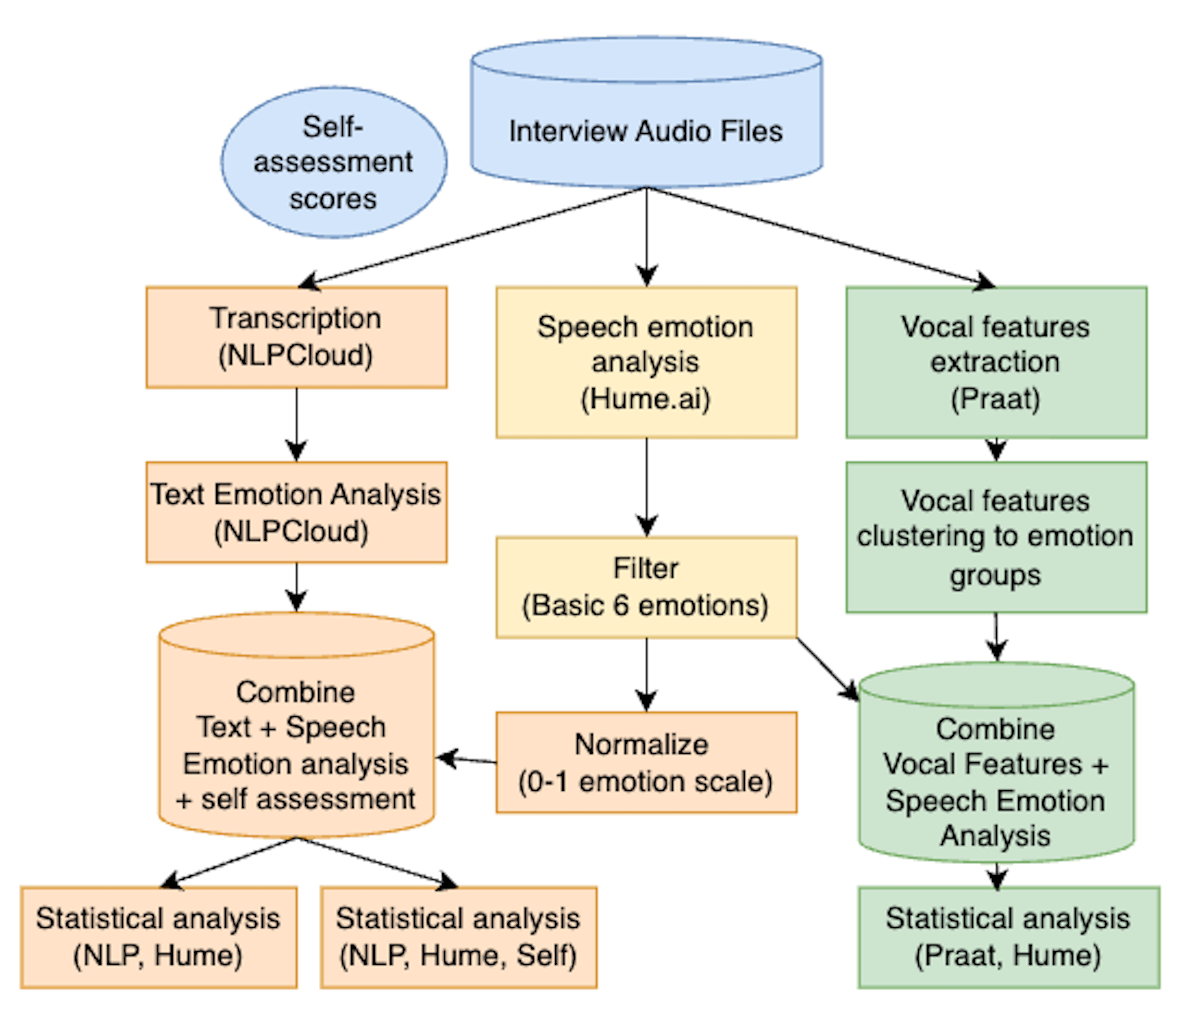
\includegraphics[width=0.8\textwidth]{png/flowchart2.png}
    \caption{The multi-modal pipeline used in this study.}
    \label{fig:pipeline}
\end{figure}


\subsection{Research Question 1}
\textbf{How does AI-model for speech emotion recognition compare to research on vocal markers for emotions in Swedish speech?}

To answer this question, speech recordings are collected from participants as they describe emotionally charged experiences. AI-based emotion recognition using Hume.ai, are used for AI-based Speech Emotion Recognition. Voice feature extraction from the recordings is made, to compare to AI-labeled emotions with known vocal markers from existing Swedish emotion research \autocite{Ekberg2023}. 

\subsection{Research Question 2}
\textbf{Can we understand the emotions from textual content of the speech, with the same data as in RQ1? }

To answer the second question, the recorded speech is transcribed and analyzed for emotion recognition using NLP Cloud’s emotion recognition to assess the emotional content of speech transcripts. The text-based AI labels are compared with speech-based AI labels to determine whether emotion is preserved in textual content alone. 

\subsection{Research Question 3}
\textbf{How do AI-generated emotion labels (speech \& text-based) compare to self-reported emotions? }

For the third question, participants complete a self-assessment survey after each interview segment, where they rate their emotional state on a 1-6 scale (1 = very weak, 6 = very strong) for relevant emotions. The self-reported emotions are compared with AI-generated labels from both speech and text models to analyze agreement and divergence. The results are clustered as agreements, partially agreements, and disagreements across methods. 


\section{Data Analysis}
To systematically evaluate the agreement between different emotion detection methods, a combination of statistical analyses and visualizations was applied for speech-based AI, text-based AI, vocal markers, and self-reported emotions. 
The analysis aimed to assess the alignment with established vocal marker research and subjective human perception, where identification and categorization of differences where analyzed. 

\subsection{Statistical Analysis Approach}
\subsubsection{RQ1: Vocal Markers vs. Speech-Based Emotion Recognition}
The first step involved applying a custom emotion categorization function based on standardized distances from the Swedish research on vocal markers \autocite{Ekberg2023}, to cluster vocal features into emotional categories. This approach adapted 
absolute standardized deviations across key acoustic features, as detailed in section \ref{sec:vocal-markers} and \ref{sec:theo-stat-analyse}. 

Following the initial clustering, correlations were calculated between: 
\begin{itemize}
    \item Individual vocal features and Hume AI emotion scores. 
    \item The categorized vocal emotion scores and corresponding vocal features. 
    \item The categorized vocal emotion scores and Hume AI emotion scores.
\end{itemize}
Limiations of the customized categorization method were identified during this phase and are discussed in the results. 

For further exploration of how vocal features varied across AI-detected emotions, one-way ANOVA tests were conducted, follwed by Tukey's HSD analysis to evaluate specifc feature differences, see \ref{sec:theo-stat-analyse} Statistic Analysis for details.  

To track changes over time, each audio recording were segmented into timeframes of around 5s including Hume AI emotion scoring and vocal features for that specific segmment. These were analyzed by tracking Z-score variations, see \ref{sec:theo-stat-analyse}, in key vocal features (pitch, intensity, jitter, and shimmer) throughout each recording. 
This enabled observation of how vocal features shifted within a single clip and to see how these changes matched Hume's emotion predictions. 

\subsubsection{Custom Emotion Categorization Method}
To complement the correlation analysis with Hume AI, a custom rule-based categorization method was integrated to group emotion probabilities from extracted vocal features. 
The approach was based on the Swedish research on vocal markers in emotions \autocite{Ekberg2023}, where statistical patterns were identified in vocal markers across five emotions: 
anger, joy, sadness, fear, and surprise. The Swedish research did not state their used baseline for neutral speech, therefore the baseline for this study is the average vocal features of all clips. 

The method functions as following: 
\begin{itemize}
    \item 1. Predefined means and standard deviations for each vocal features identified for each emotion were retrieved from the Swedish research \autocite{Ekberg2023}. These features are stored in JSON format. 
    \item 2. For every feature included in a recording, the function calculates the standardized distance between the measured vocal value and the mean for each emotion: 
    \[
    d_{\text{emo}} \, \text{+=} \, \frac{|x - \mu|}{\sigma}
    \]
    where \( x \) is the observed value, and \( \mu \), \( \sigma \) are the mean and standard deviation for the pair of feature and emotion.  
    \item 3. To increase the functionality, distances are inverted so smaller distances can result in higher emotion scores. 
    This is calculated with the function below, where \( \epsilon \) is a small constant to avoid division with zero. 
    \[
    \text{score}_{\text{emo}} = \frac{1 / (d_{\text{emo}} + \epsilon)}{\sum_{e} 1 / (d_{e} + \epsilon)}
    \]
    \item 4. The output is a normalized probability value that is distributed across all five emotions. 
\end{itemize}
The method allowed to map vocal data to emotion estimates in an interpretable way to enable structured comparison with speech-based emotion labels. 
However, the performance of this method for our dataset had limitations and gave uniform emotion labels. 

\subsection{RQ2 and RQ3: Speech-Based AI vs. Text-Based AI, AI-labels vs. Self-Assessed Emotions}
For both RQ2 and RQ3, statistical analyses were used to evaluate the alignment between AI-generated emotion scores and self-reported emotions. The following methods were applied across both research questions:
\begin{itemize}
    \item Pearson correlation coefficients and associated p-values for measurement both for single clips and the full dataset. 
    \item T-tests and calculation of Cohen's d to evaluate statistical significance and effect sizes. 
\end{itemize}
For all statistical tests, a p-value below 0.05 was considered as statistical significant, implying that the observed correlations or differences were unlikely to have occurred by chance. 
These statistical methods were applied to the entire dataset, and separately for negatively and positively oriented interview scenarios to identify potential contextual differences.
For RQ2, comparisons focused on speech-based vs. text-based AI results, and RQ3 extended the comparison to include self-reported emotions as a subjective component.

\subsection{Data Normalization}
To enable direct comparison across different sources, all emotion scores were normalized to sum up to 1. The normalization included the following steps: 
\begin{itemize}
    \item 1. Surprise combination: Hume AI predicted two seperate labels for Surprise, one positive and one negative. These were merged into a single "surprise" by calculating the average. 
    \item 2. Filtering and formatting: Filtering to only include the five target emotions (anger, joy, sadness, fear, surprise), since Hume predicted around 30 different emotions. All emotion labels were converted to lowercase. 
    \item 3. Normalization: The emotion scores were normalized so the sum of all five target emotion values equals 1. This was done by dividing each score by the total sum of the emotion values. If the total sum was zero (no emotion detected), all scores were set to 0. 
\end{itemize}
Normalization ensured consistent comparability between the sources, for both AI models and self-assessments, regardless of scale differences in raw scores. 
\subsection{Visual Analysis}
\subsubsection{RQ1:}
Visualizations included: 
\begin{itemize}
    \item Heatmaps showing correlation matrices.
    \item Line plot diagrams for the full dataset. 
    \item Bar chart diagrams for single clips. 
    \item Composite correlation diagrams. 
    \item Over-time diagrams comparing vocal features and Hume labels. 
\end{itemize}
To evaluate the performance of the custom vocal feature-based emotion categorization method, line plots and bar charts were implemented to visualize differences between the generated scores and Hume AI's predictions. 
The line plot summerizes average emotion scores across the full dataset, while bar charts presented detailed comparisons for individual audio recordings. 
These diagrams emphasizes deviations and alignments between the categorized vocal marker method and AI-based emotion prediction. 

Composite correlation diagrams were used to explore associations between single vocal features and AI-generated emotion scores. 
For these diagrams, Pearson correlation coefficients were calculated for each emotion and its relation to pitch and intensity, the results are visualized as grouped bar charts to easily identify positive or negative tendencies. 

\subsubsection{RQ2 and RQ3:}
Visual methods included: 
\begin{itemize}
    \item Difference bar charts to illustrate the average difference in Hume AI and NLP Cloud's emotion scores for each emotion category, to provide a clear view of systematic deviations. 
    \item Grouped bar charts to present average emotion scores from both AI systems, seperated by interview sentiment (positive vs. negative), to explore variations in emotion detection depending on the interview context. 
    \item Scatter plots (RQ3) to explore detailed relationships between AI-based emotion scores and self-reported emotions for single emotions and recordings.
\end{itemize}
These visualizations were integrated to support the identification of alignment patterns between the AI systems, and contributed with insights into how the modality of the AI influences emotion recognition results. 
Python have been utilized to create all visualizations. 

Given the limited dataset size and timeframe, a combination of statistical methods and visual analysis, was utilized to balance quantitative data with qualitative interpretation and support the exploratory nature of this study. 

\section{Model Configuration}
\subsection{NLP Cloud}
\label{sec:method-nlp}
The text-based emotion recognition is classified with NLP Clouds finetuned-llama-3-70b model
through prompting, which allows a more flexible approach.
Each text input uses the following prompt:
\begin{center}
    \begin{minipage}{0.7\textwidth} 
    \begin{lstlisting}[language=json, caption={NLP Cloud configuration prompt.}]
        prompt = (
            "You are an emotion analysis system. "
            "Given a Swedish text, respond only with a JSON object using these emotion
            labels: "
            "joy, surprise, fear, anger, sadness. Each value must be a float
            between 0.0 and 1.0. "
                "Respond with the JSON directly and nothing else.\n\n"
                f"{text}"
            )
    \end{lstlisting}
    \end{minipage}
\end{center} 
The prompt that is used returns a JSON response with float values ranging from 0.0 to 1.0 for each of
the emotions with the labels “joy”, “surprise”, “fear”, “anger”, “disgust” and “sadness”. This approach
was chosen to ensure these specific emotions being analyzed due to them being the feelings of the basic
six, which are the feelings used in the research about acoustic features in swedish speech done by
Ekberg \autocite{Ekberg2023}. 

\subsection{Hume AI}
To ensure consistency across the different models used in this research, some changes have been
made to adjust the output from the Hume AI model to better match the format used in NLP Cloud.
Additionally, NLP Cloud has the feeling surprise while Hume has two different feelings for surprise,
the two being positive surprise and negative surprise. Therefore, the scores of the two feelings of
surprise from the Hume model have been combined in this research to give just one number that
creates the average of the two to match the format.

\section{Validity and Reliability}
\subsection{Validity}
To ensure validity, the interview scenarios are pilot tested to ensure they provoke intended emotions \autocite{Bryman2022}. The use of multiple AI models (speech- and text-based) allows for cross-validation of results. Standardized interview prompts ensure consistency across participants. Participant self-assessment serves as a secondary reference to evaluate AI-labeled emotions. Triangulation across AI, vocal markers, text analysis, and self-assessments enhance convergent validity \autocite{Creswell2023}. 

\subsection{Reliability}
To ensure reliability, standardized equipment and scenario are used to ensure replicability. Hume.ai, NLP Cloud, and Praat provide consistent measures. The AI models used in the study (Hume.ai and NLP Cloud) are pre-trained and validated emotion recognition systems. Correlation will be determined and are used to quantify the reliability of AI models in detecting emotions. The study has a replicable experimental setup, with documentation supporting replication to allow researchers to reproduce similar evaluations.  

Triangulation is achieved in the study through comparison of speech AI, text AI, and self-reports which improves creditability. Any discreteness will be analyzed qualitatively to contextualize potential biases rather than assuming errors. 
Reliability is ensured through standardization in data collection. All interviews are preprocessed to reduce background noise and normalize volume levels. The online tool Auphonic \autocite{Auphonic} is used for this, due to its simple usability for noice reduction, ability to cut out pauses and limit loudness. The same data processing steps are applied consistently for all recordings, ensuring equality in analysis. The study has a replicable experimental setup, with usage of pre-trained, publicly available APIs, and documentation supporting replication to allow researchers to reproduce similar analyses. These measures ensure that our study is generalizable within the scope or automated emotion recognition for stress analysis. 

\section{Considerations}
To consider the implications of this study, several factors must be recognized. To address ethical and privacy concerns, all participant data is anonymized and securely stored to ensure privacy. The participants provide informed consent before engaging in this study. The emotion-provoking scenarios are designed to minimize distress, focusing on natural, everyday emotions rather than triggering events. The participants will have scenarios to choose from, see 2.2 Data Collection. 

Scientific considerations extend to emotion research to Swedish speech and AI tools. Findings in the study can inform future human-interaction research in emotion-based applications. Societal considerations include that the insights could enhance AI-driven mental health tools and future research, especially for Swedish language and real-world interviews. 

\chapter{Theoretical Framework}
\label{chap:theoretical-framework}

The following chapter will introduce the relevant theories and key concepts related to emotion recognition, such as speech-based and text-based models and technologies. 
This chapter will explain how vocal features and speech prosody can help to identify different emotions in spoken languages, using different AI tools and software. This study aims to compare accuracy and effectiveness of different approaches by conducting interviews and collecting data, which will be analyzed using a Python application. The elements of the Python application for analyzing the data from the interviews will be comprehensively explained in this chapter.

\section{Affective Computing}

 Affective computing was introduced by Professor Rosalind Picard in the mid-1990s to early 2000s \autocite{Tian2022}. By exploring the ways in which human emotions are recognized, understood and expressed through different forms of behaviors and communication, the domain of affective computing is a field that merges the principles of artificial intelligence with insights from social and behavioral science \autocite{Tian2022}.

\section{Natural Language Processing and Emotion Recognition}

 The first English language lexical database was created in 1998 \autocite{Kusal2023} for Natural Language Processing (NLP) tasks. The term sentiment and emotional analysis came to practice in 2001 \autocite{Kusal2023} to predict the stock market. In 2005, the first article was written on emotion and opinion detection from text. Concept-level sentiment analysis resources were publicly available in 2009. Word embedding is the term to represent words for NLP text analysis and was developed in 2013, the same year as neural network first was adopted in NLP tasks. The field had a massive upwelling when the transformers concept was published in 2017, followed by the evolution of BERT, a pretrained model that automated text analysis and classification in 2018 \autocite{Kusal2023}. 

Traditional approaches for sentiment analysis classification have been used since the past few decades, which rely on rule-based methods such as “bag of words” method to process text. The method represents text based on word frequency without consideration of word order. It can identify sentence structure, negation, emphasis, subjectivity and irony. Recent models leverage deep learning algorithms that process raw text by first cleaning and pre-processing it, including punctation, stop words and markups, as well as applying stemming (the process of reducing words to their root form by removing prefixes or suffixes to simplify text analysis in NLP) \autocite{Kansara2020}. 

 Deep learning applicate artificial neural networks (ANN) to learn tasks using multiple layers of network. In traditional models only one or two layers could be used, but in deep learning much more learning power of artificial neural networks is exploited \autocite{Zhang2018}. Studies have shown consistently higher accuracy for sentiment analysis using deep learning algorithms compared to traditional machine learning algorithms \autocite{Kansara2020}.

 Traditionally, SER systems are comprised of three components: signal preprocessing, feature extraction, and classification \autocite{Sahoo2023}.

Emotion recognition from speech is generated by other types of machine learning algorithms, some algorithms are used for both types of emotion recognition, where Support Vector Machine (SVM) have shown high accuracy for speech analysis. 

SVM is a simple machine learning algorithm that is highly preferred, since it requires less computational power for producing substantial accuracy \autocite{Kusal2024}.

 

\section{Speech-Based Emotion Recognition}

 In the field of artificial intelligence, researching areas to be able to identify emotions is important to read humans better. Studies about speech-based emotion recognition (SER) have been ongoing since 1978 \autocite{LGENSNMEZ2024}. SER identifies how something is being said without the context of the words spoken. These systems are used in many different areas, most often in areas of interactions between humans and machines (Zhang, 2025). 

 Although there is a wide range of SER-algorithms, some approaches using more complex setups that involve Convolutional Neural Networks (CNN) based SER algorithms among others \autocite{Ri2023}, the process of a SER algorithm could look like figure \ref{fig:stages-SER}, involving several steps as feature extraction, selection and classification.


\begin{figure}[ht]
    \centering
    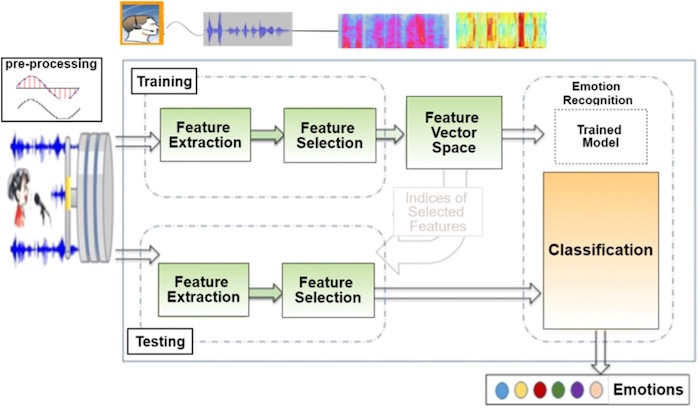
\includegraphics[width=10cm]{png/Figure 4-Stages in SER.jpg}
    \caption{\textit{An overview of the stages in SER to analyze speech data for emotion detection} \autocite{LGENSNMEZ2024}}
    \label{fig:stages-SER}
\end{figure}
 

 While emotions can be recognized via many channels such as speech, facial expressions and text, speech signals are rapid and natural which makes vocal audio fitting for emotion recognition. According to \autocite{LGENSNMEZ2024} there are several key benefits with SER:

\begin{itemize}
    \item There is only a small amount of hardware needed to capture vocal data.
    
    \item It is a simple process to collect vocal data, due to little hardware being needed.
    
    \item It is harder to mimic vocal data compared to facial data.

    \item Vocal data is less demanding in terms of storage than video footage for example.

    \item Participants in SER experiments may feel more comfortable with vocal analysis than face analysis in terms of confidentiality, resulting in datasets reflecting real emotions more accurately.
\end{itemize}

 

\subsection{Hume AI }

Hume is a technology company dedicated to advancing the field of emotion recognition.

Having conducted extensive psychology studies to explore human emotions and the way these emotions are expressed, Hume AI has used the research to develop advanced machine learning models \autocite{HumeAi-aboutScience} as well as using deep learning for the research and development \autocite{Brooks2023}.

 The official website of Hume AI outlines several influences on their emotional mapping. Drawing influence from key figures such as David Hume, Charles Darwin and Paul Ekman, Hume AI’s research is grounded in these foundational theories of emotions. Paul Ekman’s “The Basic 6” is mentioned \autocite{HumeAI-AboutHume} and remains relevant throughout this research. 

 One of the measurements used to recognize emotions in vocals with Hume AI in this research is speech prosody. 

Speech prosody gives crucial insights into a speaker’s purpose in their communication. Particular emotions and the intensity of those emotions are indicated with intonation, rhythm and pitch of the speaking voice \autocite{Thompson2004}\autocite{Tomasello2022}. It simply refers to the patterns and tone in the speech that are not related to the actual words being spoken \autocite{Cowen2019}.

Happiness and sadness show the opposite characteristics of each other, where happiness is linked to quicker tempo and higher pitch while sadness has the opposite, a slower tempo and lower pitch. The clear difference between the characteristics serves as the difference in the speech prosody of the two emotions \autocite{Thompson2004}. 

 In figure \ref{fig:hume-ai-speech-prosody}, a visual presentation of Hume AI’s speech prosody model is visible \autocite{HumeAIProsody}. Emotions are clustered with other similar emotions, one example being amusement and joy, or distress and anxiety.
\begin{figure}[ht]
    \centering
    \includegraphics[width=10cm]{png/Figure 5-Hume AI’s speech prosody.jpg}
    \caption{\textit{Visual representation of Hume AI’s speech prosody model} \autocite{HumeAIProsody}}
    \label{fig:hume-ai-speech-prosody}
\end{figure}

 To ensure a broader range of emotion recognition with a more comprehensive analysis of human voices in this research, speech prosody is used in combination with another measurement, vocal bursts.

Vocal bursts play a key role in social communication between humans. They are short emotional sounds which occur naturally, some examples being laughs, sighs or cries \autocite{Brooks2023}.

Vocal burst and voice overall have been relatively overlooked in the fields of machine learning and affective computing due to more focus being held on facial expressions. Even if speech prosody has been studied more extensively, there has been newer research showing that vocal bursts convey more than ten different emotions with consistency, being mostly consistent across different cultures as well \autocite{Baird2022}.

 Figure \ref{fig:hume-ai-vocal-burst} shows Hume AI’s mapping of non-verbal communication, vocal bursts \autocite{HumeAIVocalExpression}. Emotions are shown and as well as in Hume AI’s speech prosody model, the emotions are clustered indicating some emotions are more associated with each other.

\begin{figure}[ht]
    \centering
    \includegraphics[width=10cm]{png/Figure 6-Hume AI’s vocal burst.jpg}
    \caption{\textit{Visual representation of Hume AI’s vocal burst model} \autocite{HumeAIVocalExpression}}
    \label{fig:hume-ai-vocal-burst}
\end{figure}

 While there are other tools for emotion recognition, Hume AI seems to be among the few that are specifically designed for Voice AI while being able to recognize emotions through specifically speech prosody and vocal burst with no need to finetune it yourself. Using models needing finetuning would not fit the scope of this thesis given the limited timeframe, and while models like OpenAI whisper is an extensively trained model on hundreds of thousands of hours on data, their main focus leans toward transcribing speech \autocite{OpenAI2022}.

\subsection{Praat Parselmouth}

In the field of software for analyzation in linguistics, Praat is a well-established tool to analyze different elements in speech. Being able to estimate elements such as fundamental frequency and intensity among others, Praat holds a broad spectrum of algorithms in acoustics, being a successful tool for analyzing acoustics \autocite{Jadoul2024}.

 

 

Designed to provide efficient access to the core functionalities of Praat in Python for programmers, Parselmouth is an open-source Python library \autocite{Jadoul2018}.

Python is widely used for data analysis, but it had been noted that there were challenges with analyzing acoustics in Praat, this due to the functionality often being missing or scattered across multiple incompatible libraries.

 Parselmouth streamlines and optimizes workflows in a single programming environment by enabling a deeper integration of the capabilities of Praat in combination with other libraries \autocite{Jadoul2024}. Not designed to replace Praat, but rather a way to enable users to access the functionality of Praat directly in Python, the main objectives in Parselmouth according to \autocite{Jadoul2018} are:

 \begin{itemize}
     \item Enable users already experienced with Praat to effectively incorporate its functionality with Python’s scientific tools, being tools that are not obtainable in Praat.
     \item Providing Python users with the ability to utilize the functionality of Praat, even if they are not experienced users of it.
     \item Enhancing the optimal aspect of workflow for users preferring to conduct their work within a single programming language.

 \end{itemize}
 
 The benefits of Parselmouth both in terms of the usage for completing this thesis and overall, are it being open source and compatible with Python as Python is widely utilized and backed by a vast community of researchers and engineers, among others. Parselmouth integrates the different strengths of different approaches to provide a truly pythonic library, behaving consistently with other well-known Python libraries.

Parselmouth directly utilizes the official C/C++ source code of Praat instead of having to reconstruct its algorithms. This simplifies the process since it guarantees full consistency with Praat without the requirement of learning its scripting language \autocite{Jadoul2018}.

There are other similar tools that essentially could accomplish the same task, like Librosa although it is more tailored for both audio and music analysis. It does have feature extraction \autocite{Babu2021}, but the decision on which software to use for linguistic analyzation still falls on Praat Parselmouth due to it being more fitting for the purpose of this thesis.

 

\section{Text-Based Emotion Recognition}

In the field of NLP, the comprehension of the context behind words in text-form has gone from only being able to determine the tone in text to actually identifying the emotions behind them \autocite{Esfahani2024}, recognizing these capabilities has valuable practical applications in enhancing different domains within human-computer interaction \autocite{Shelke2022}.

 Text-based emotion detection relies on four main approaches, according to \autocite{Kusal2023} written in 2023:

 \begin{enumerate}
     \item Keyword-based: Matches words in a text with predefined emotion keywords from resources like WordNet, adjusting for intensity and negation.
     \item Rule-based: Uses linguistic rules and probabilistic affinity to classify emotions after preprocessing.
     \item Machine learning-based: applies supervised or unsupervised models to classify emotions, extracting key features from preprocessed text.
     \item Deep learning-based: utilizes neural networks to learn complex patterns from tokenized and embedded text data for emotion classification.
 \end{enumerate}

Machine learning classifiers are significantly used in text-based classification, since they use labeled datasets and are therefore data driven. Machine learning models are trained on large number of datasets and learn from experience, with classifiers that contain labels for input and desired output. Transformer-based models, such as BERT, are based on machine learning models which are trained on vast amounts of data and can be fined-tuned for specific tasks. BERT is a deep learning model based on attention processing. It gains a thorough text-understanding through considering left and right contexts equally. The model solves NLP issues and is used to train general language models on large datasets \autocite{Kusal2024}.

\subsection{NLP Cloud}

There are limited publicly available APIs for text-based emotion detection. The decision to use NLP Cloud has several reasons. Compared to other available TBED APIs, that do not require pre-training, NLP Cloud has comprehensive documentation for both API and the models it is based on. The company has support as well as information about Data Privacy and Security \autocite{NLPCloud}, which also other APIs for TBED has. For example, Vern AI (AI, u.d.) provides customer support but has very limited information about the API or documentation that is easily accessible. TwinWord \autocite{TwinWord} was another choice, also providing contact support and privacy information, but was deficient in comprehensive documentation and limited information about the API. 

 NLP Cloud was the obvious choice for several reasons. In addition to what is mentioned above, the company has solid customers like Zoom and collaboration with Nvidia. They provide information about what models they use for their API which can be downloaded and fine-tuned if desired. In contrast to the other APIs, NLP Cloud provide APIs for Speech-to-Text transcription, and they have an emotional analysis model supporting Swedish Language. Therefore, no translation is required beforehand. Their speech-to-text API is based on OpenAI’s Whisper model \autocite{NLPCloud}. OpenAI provides a research report on the model, which is a speech recognition system designed to process and transcribe audio with remarkable robustness and generalization. Contrasting traditional models that heavily rely on unsupervised pre-training or dataset-specific fine-tuning, Whisper leverages large-scale weakly supervised training from over 600,000 hours of multilingual audio data. This includes 96 languages beyond English. Whisper handles several tasks, for instance speech recognition, language identification, and translation \autocite{Radford2022}. 

 For sentiment and emotion analysis, NLP Cloud provides several options. Two of them are equally researched with relatively comparable results. DistilBERT Base Uncased Emotion is one option, with studies on DistilBERT, and Transformer-model which require finetuning and require less computational resources than traditional BERT (Bidirectional Encoder Representations from Transformers) models. The model was developed by Google AI Language researchers in October 2018. BERT has challenges regarding fixed input length and computational complexity, reasons that led to DistilBERT’s development in October 2019. This pre-trained model uses technology that accomplishes to reduce a BERT model by 40\% while preserving 97\% of language understanding capabilities 60\% faster. The model accuracy for sentiment analysis ranges from 95.7\% to 96.6\% on Yelp Open Dataset, which has been demonstrated as a valuable resource of sentiment-labeled review-data \autocite{Areshey2024}. NLP Cloud provides a pre-fine-tuned version of DistilBERT. However, it does not support Swedish language and translation beforehand is necessary for this study. A fine-tuned version of Llama 3 is an option on NLP Cloud that support several languages including Swedish \autocite{NLPCloud}. Opposed as to DistilBERT, some studies on emotion detection have been conducted on Llama 3. Both models have predominantly been evaluated for sentiment analysis. Emotion identification using Llama 3 showed an F1 score of 0.48 as average for all tested emotions: anger, joy, sadness, surprise, fear, and love \autocite{Zhang2024}. A fine-tuned version of Llama 3 was tested for sentiment analysis, which resulted in an accuracy increase from 0.333 to 0.923 and F1 score from 0.50 to 0.91. The authors of this study imply that these results are superior performance against other models that are included for comparison, including DistilBERT \autocite{Kumar2024}. In a text classification study, mainly examines speed performance, DistilBERT had an accuracy between 0.94-0.96 for the Amazon Alexa Reviews dataset but 0.35-0.41 for the Brexit Blog Corpus dataset \autocite{SilvaBarbon2022}. As for many models for emotion recognition mentioned in this report, the dataset affects the results heavily. 

 Regarding multiple language performance, a study examined LLaMA 3 vs. State-of-the-Art Large Language Models on their ability to detect fake news. Two datasets were tested, one Romanian and one English. Their proposed Llama 3 model accomplished higher precision and accuracy across several metrics in fake new detection. For the English dataset, the fine-tuned Llama 3 model had lower accuracy compared to ChatGPT 4 and Gemini. Yet, it outperformed these models for the Romanian dataset. The study also explored their fine-tuned Llama model compared to its base version. The fine-tuned model outperformed earlier models in distinguishing nuanced categories, particularly for the Romanian dataset where it achieved a remarkably high accuracy of 68\% in one category \autocite{Repede2024}.

 Comparing these two alternatives for text-based emotion detection in Swedish, the fine-tuned Llama 3 model emerges as the most suitable choice. Although the exact fine-tuned version of the model available on NLP cloud has not been publicly researched, its built-in compatibility with Swedish, combined with research on a Romanian dataset, makes it a stronger candidate than DistilBERT. Both models have achieved high accuracy for TBED. Nevertheless, given this study is aimed to focus on emotion recognition models for Swedish speech, the Llama model without need for prior translation is a more valuable choice. 

 

\section{Vocal Markers}
\label{sec:vocal-markers}

 States of emotions are determined by many different factors, but in speech, different vocal markers such as prosody, pitch and loudness are among the telling features when it comes to emotions \autocite{Ekberg2023}, where frequency is perceived as pitch, while amplitude is heard as loudness \autocite{Frhholz2019}.

In this research vocal markers are crucial to understand the difference in certain emotions in voice.

 Figure \ref{fig:compare-acoustic-parameters} \autocite{Ekberg2023} shows a table of comparisons with certain parameters of vocal markers measured for five different emotions in the Swedish language and some explanations for the different parameters. This is used in this thesis as a comparison for the vocal markers collected from the interview data in the conducted experiment, although this thesis does not use all acoustic features to measure emotions.
 
\clearpage
\begin{figure}[ht]
    \centering
    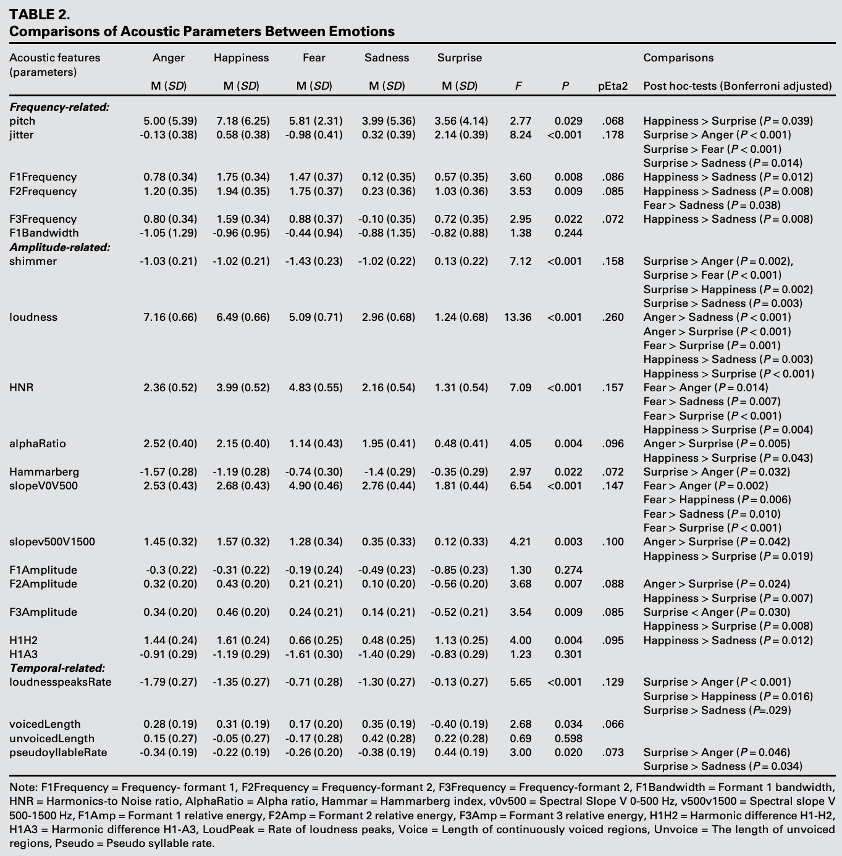
\includegraphics[width=10cm]{png/Figure 7- Table comparing acoustic parameters.png}
    \caption{\textit{Table comparing acoustic parameters between emotions} \autocite{Ekberg2023}}
    \label{fig:compare-acoustic-parameters}
\end{figure}

 Figure \ref{fig:acoustic-variations} shows a table of variations in different emotions measuring the acoustic parameters pitch, intensity, speaking rate and voice quality which are often used to identify emotions \autocite{Khalil2019}. Although figure 3.4 displays a wider variety of more specific acoustic features, figure 3.5 provides a foundational understanding of different acoustic features connected to the different emotions.

\begin{figure}[h]
    \centering
    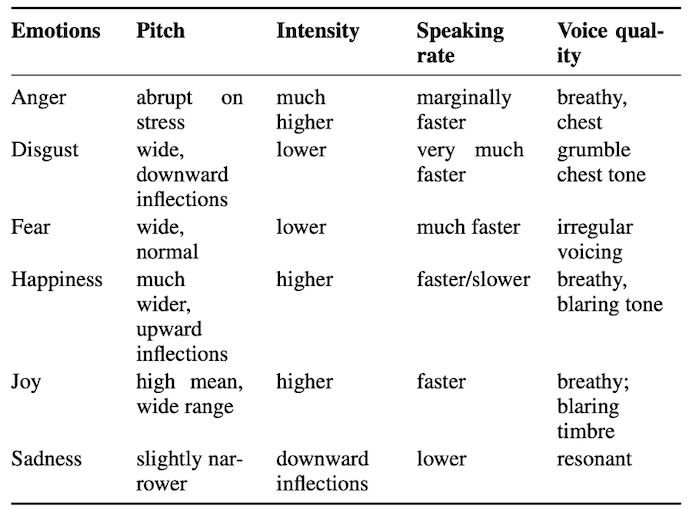
\includegraphics[width=8cm]{png/Figure8-AcousticVariations.png}
    \caption{\textit{Acoustic variations in different emotions} \autocite{Khalil2019}.}
    \label{fig:acoustic-variations}
\end{figure}

\section{The Experiment}

An experiment will be conducted and will consist of short interviews with voluntary people. These interviews will be recorded for data collection and will be used to extract emotions with a Python application. 

\subsection{Python Application}

The Python application serves as the central system for processing and analyzing emotions in speech and will integrate several tools and frameworks to extract emotions.

The steps for the process consist of:

\begin{enumerate}
    \item Audio recording
    \item Feature extraction
\end{enumerate}

\begin{itemize}
    \item Prosody and vocal bursts will be analyzed with Hume AI to detect emotional cues from pitch, intonation and vocal bursts using Hume AI’s models.
    \item Extracting vocal features such as jitter, shimmer and frequency with Praat Parselmouth.
    \item Convert speech to text and analyze emotions in text with NLP Cloud.
\end{itemize}


\subsection{Interviews and Surveys}

The interviews involve voluntary participants engaging in short audio-recorded interviews, designed to draw out natural emotional responses. The participants will be asked questions to prompt them to recall and reflect on past experiences which encourages them to revisit emotions they felt at that time. 

For ethical purposes the participants will be given a selection of topics to choose from, minimizing the risk of discomfort or distress. The audio recordings will be anonymous and recorded in a controlled acoustic environment to ensure minimal noise interference.

Questions asked during the interview follow one of many emotion induction techniques, “autobiographical recall”. This is a method used to facilitate the re-experiencing of emotions felt in a previous moment \autocite{Siedlecka2019}, which is what is intended for the interviews to be able to collect emotional data from vocal recordings. By letting the participant think and speak about a memory from the past, emotions felt in that moment reflect in their voice.

 After the interview is done, the participants will answer a survey doing a self-assessment of their emotions felt during the interview. This will enable a comparison between emotion detection and the participants reported emotional experiences.

There are many different methods for self-assessment, and emotional self-assessment is linked to many different theories. Many are connected to emotional intelligence (EI), trait emotional intelligence (trait EI) and Core Self Evaluation (CSE) \autocite{Montasem2013}, but rather than conducting a comprehensive exploration of different psychological theories in self-assessment, this research will use simplified surveys at a basic level for the purpose of fulfilling the technical objectives of the work. 

 The theories behind the interviews are stated in the possibility of detecting emotions in voices. While there are a lot of recognized emotions that can be detected in different AI models and software tools, the interview will focus on bringing out two different basic emotions to maintain a manageable scope, while ensuring ethical feasibility.

Research has stated that there are different levels of unique universal signs for different affective states and while there are evidence supporting the universality for certain emotions such as anger, fear, surprise, sadness, happiness and more, there are also emotions that do not include all characteristics that distinguish them from other mental states, two examples being guilt and shame \autocite{Ekman2011}. Research of this nature supports the rationale for having the focus solely on two of the basic emotions for this thesis. The questions in the interviews will focus on bringing out two separate emotions, one on the positive spectrum, happiness, and one on the negative spectrum, anger.



\section{Statistical Analysis}
\label{sec:theo-stat-analyse}

\subsubsection{Pearson Correlation Coefficient}
Pearson's r is a measurement of the strength and direction of a linear relationship between two variables. The value range is from -1 to 1, where positive values implies a positive correlation and negative values the opposite.
Values close to +-1 indicate a strong correlation, values between +-0.30 and +-0.49 a moderate correlation, and values 
below +-0.29 are seen as a weak correlation. Values around 0 implies no linear correlation \autocite{Bruce2017}.

\subsubsection{P-Value}
A p-value indicates if the observed results have a probability of occurance by chance. A widely accepted threshold for statistical significance 
is p < 0.05, which means there is less than a 5\% possibility that the observed effect is random \autocite{Bruce2017}. 

\subsubsection{Z-score Standardization}
Acoustic features such as pitch, intensity, jitter and shimmer can have great variation. To ensure comparability in statistical analyses, features are often standardized using Z-score standardization \autocite{Ekberg2023}.
This method transform data to have a mean of zero and a standard deviation of one, ensuring meaningful comparisons across features. By this, a variable does not have an overly influence due to a scale of the measurement. 
The measurements are described as "standard deviations away from the mean". \autocite{Bruce2017}. 

\subsubsection{Standardized Distance for Emotion Categorization}
Emotion categorization based on vocal features can be operated through standardized distance methods, where deviations from the baseline of acoustic profiles are quantafied. Using standardized differences allow an interpretable measure of how vocal features aligns with expected patterns for each emotion \autocite{Ekberg2023} \autocite{Bruce2017}. 
The categorization method used in this study is a custom method inspired by this standard practice. 

\subsubsection{ANOVA Tests}
ANOVA (Analysis of Variance) is a standard statistical method used to determine if there are any significant differences in means across multiple groups {Bruce2017}. It is used to categorize grouping factors and are one method in the Swedish research for vocal markers {Ekberg2023}.  

\subsubsection{Tukey's HSD}
When ANOVA presents significant differences between group means, Tukey's HSD test is incorporated as a post analysis to identify which groups are divergent from each other. 
This method controls for errors when making multiple comparisons \autocite{Bruce2017}. 
\subsubsection{T-Tests and Cohen's d}
Paired T-tests are used to compare the means between two groups to determine statistical significance, while Cohen's d provides a standardized measure of the effect size which indicates the magnitude of the observed differences \autocite{Cohen1977} \autocite{Bruce2017}.
\chapter{Results}
\label{sec:results}


\section{Presentation of Collected Data}
\subsection{Overview of Interviews}
We conducted semi-structured interviews with 16 native Swedish speakers (10 M/6F, age 23-78), each lasting 1-3 minutes. Each participant was interviewed for two different scenarios, resulting in 30 different recordings. All interviews were audio-recorded in a quiet room and elicited two target emotions – anger and happiness – via open-ended prompts (e.g. “Is there anything in society that makes you upset? What? How does that make you feel?”; “Can you remember one time you felt really proud of yourself?”). The participants rated their perceived emotions on a 1-6 scale immediately after each scenario. The rated emotions covered the basic 5 emotions mentioned in this report: anger, joy, sadness, fear, and surprise. 

Table~\ref{tab:interview_table} presents the participants ID, gender, age, and self-assessed scores for their perceived emotions for respective interview scenario.
\begin{table}[H]
    \centering
    \begin{tabular}{|lrl|
    >{\columncolor[HTML]{FBE2D5}}l 
    >{\columncolor[HTML]{FBE2D5}}l 
    >{\columncolor[HTML]{FBE2D5}}l 
    >{\columncolor[HTML]{FBE2D5}}l 
    >{\columncolor[HTML]{FBE2D5}}l |
    >{\columncolor[HTML]{DAF2D0}}l 
    >{\columncolor[HTML]{DAF2D0}}l 
    >{\columncolor[HTML]{DAF2D0}}l 
    >{\columncolor[HTML]{DAF2D0}}l 
    >{\columncolor[HTML]{DAF2D0}}l |}
    \hline
    \multicolumn{3}{|c|}{Participant}                                                                                                 & \multicolumn{5}{c|}{\cellcolor[HTML]{F7C7AC}Negative}                                                                                                                                                     & \multicolumn{5}{c|}{\cellcolor[HTML]{B5E6A2}Positive}                                                                                                                                                                                                  \\ \hline
    \multicolumn{1}{|l|}{\cellcolor[HTML]{D9D9D9}ID} & \multicolumn{1}{l|}{\cellcolor[HTML]{D9D9D9}M/F} & \cellcolor[HTML]{D9D9D9}Age & \multicolumn{1}{l|}{\cellcolor[HTML]{FBE2D5}A} & \multicolumn{1}{l|}{\cellcolor[HTML]{FBE2D5}J} & \multicolumn{1}{l|}{\cellcolor[HTML]{FBE2D5}Sad} & \multicolumn{1}{l|}{\cellcolor[HTML]{FBE2D5}F} & Sur & \multicolumn{1}{c|}{\cellcolor[HTML]{DAF2D0}A} & \multicolumn{1}{c|}{\cellcolor[HTML]{DAF2D0}J} & \multicolumn{1}{c|}{\cellcolor[HTML]{DAF2D0}Sad} & \multicolumn{1}{c|}{\cellcolor[HTML]{DAF2D0}F} & \multicolumn{1}{c|}{\cellcolor[HTML]{DAF2D0}Sur} \\ \hline
    \multicolumn{1}{|l|}{1}                          & \multicolumn{1}{r|}{M}                           & 23                          & \multicolumn{1}{l|}{\cellcolor[HTML]{FBE2D5}5} & \multicolumn{1}{l|}{\cellcolor[HTML]{FBE2D5}1} & \multicolumn{1}{l|}{\cellcolor[HTML]{FBE2D5}3}   & \multicolumn{1}{l|}{\cellcolor[HTML]{FBE2D5}1} & 1   & \multicolumn{1}{l|}{\cellcolor[HTML]{DAF2D0}1} & \multicolumn{1}{l|}{\cellcolor[HTML]{DAF2D0}6} & \multicolumn{1}{l|}{\cellcolor[HTML]{DAF2D0}1}   & \multicolumn{1}{l|}{\cellcolor[HTML]{DAF2D0}1} & 4                                                \\ \hline
    \multicolumn{1}{|l|}{2}                          & \multicolumn{1}{r|}{M}                           & 26                          & \multicolumn{1}{l|}{\cellcolor[HTML]{FBE2D5}6} & \multicolumn{1}{l|}{\cellcolor[HTML]{FBE2D5}1} & \multicolumn{1}{l|}{\cellcolor[HTML]{FBE2D5}3}   & \multicolumn{1}{l|}{\cellcolor[HTML]{FBE2D5}4} & 1   & \multicolumn{1}{l|}{\cellcolor[HTML]{DAF2D0}1} & \multicolumn{1}{l|}{\cellcolor[HTML]{DAF2D0}6} & \multicolumn{1}{l|}{\cellcolor[HTML]{DAF2D0}1}   & \multicolumn{1}{l|}{\cellcolor[HTML]{DAF2D0}2} & 1                                                \\ \hline
    \multicolumn{1}{|l|}{3}                          & \multicolumn{1}{r|}{F}                           & 27                          & \multicolumn{1}{l|}{\cellcolor[HTML]{FBE2D5}4} & \multicolumn{1}{l|}{\cellcolor[HTML]{FBE2D5}1} & \multicolumn{1}{l|}{\cellcolor[HTML]{FBE2D5}6}   & \multicolumn{1}{l|}{\cellcolor[HTML]{FBE2D5}1} & 2   & \multicolumn{1}{l|}{\cellcolor[HTML]{DAF2D0}1} & \multicolumn{1}{l|}{\cellcolor[HTML]{DAF2D0}6} & \multicolumn{1}{l|}{\cellcolor[HTML]{DAF2D0}1}   & \multicolumn{1}{l|}{\cellcolor[HTML]{DAF2D0}1} & 3                                                \\ \hline
    \multicolumn{1}{|l|}{4}                          & \multicolumn{1}{r|}{M}                           & 29                          & \multicolumn{1}{l|}{\cellcolor[HTML]{FBE2D5}2} & \multicolumn{1}{l|}{\cellcolor[HTML]{FBE2D5}1} & \multicolumn{1}{l|}{\cellcolor[HTML]{FBE2D5}3}   & \multicolumn{1}{l|}{\cellcolor[HTML]{FBE2D5}2} & 1   & \multicolumn{1}{l|}{\cellcolor[HTML]{DAF2D0}1} & \multicolumn{1}{l|}{\cellcolor[HTML]{DAF2D0}4} & \multicolumn{1}{l|}{\cellcolor[HTML]{DAF2D0}2}   & \multicolumn{1}{l|}{\cellcolor[HTML]{DAF2D0}2} & 2                                                \\ \hline
    \multicolumn{1}{|l|}{5}                          & \multicolumn{1}{r|}{F}                           & 28                          & \multicolumn{1}{l|}{\cellcolor[HTML]{FBE2D5}4} & \multicolumn{1}{l|}{\cellcolor[HTML]{FBE2D5}1} & \multicolumn{1}{l|}{\cellcolor[HTML]{FBE2D5}4}   & \multicolumn{1}{l|}{\cellcolor[HTML]{FBE2D5}1} & 2   & \multicolumn{1}{l|}{\cellcolor[HTML]{DAF2D0}1} & \multicolumn{1}{l|}{\cellcolor[HTML]{DAF2D0}5} & \multicolumn{1}{l|}{\cellcolor[HTML]{DAF2D0}1}   & \multicolumn{1}{l|}{\cellcolor[HTML]{DAF2D0}1} & 5                                                \\ \hline
    \multicolumn{1}{|l|}{6}                          & \multicolumn{1}{r|}{M}                           & 25                          & \multicolumn{1}{l|}{\cellcolor[HTML]{FBE2D5}2} & \multicolumn{1}{l|}{\cellcolor[HTML]{FBE2D5}2} & \multicolumn{1}{l|}{\cellcolor[HTML]{FBE2D5}1}   & \multicolumn{1}{l|}{\cellcolor[HTML]{FBE2D5}1} & 1   & \multicolumn{1}{l|}{\cellcolor[HTML]{DAF2D0}1} & \multicolumn{1}{l|}{\cellcolor[HTML]{DAF2D0}3} & \multicolumn{1}{l|}{\cellcolor[HTML]{DAF2D0}1}   & \multicolumn{1}{l|}{\cellcolor[HTML]{DAF2D0}1} & 1                                                \\ \hline
    \multicolumn{1}{|l|}{8}                          & \multicolumn{1}{r|}{M}                           & 27                          & \multicolumn{1}{l|}{\cellcolor[HTML]{FBE2D5}3} & \multicolumn{1}{l|}{\cellcolor[HTML]{FBE2D5}1} & \multicolumn{1}{l|}{\cellcolor[HTML]{FBE2D5}2}   & \multicolumn{1}{l|}{\cellcolor[HTML]{FBE2D5}1} & 2   & \multicolumn{1}{l|}{\cellcolor[HTML]{DAF2D0}1} & \multicolumn{1}{l|}{\cellcolor[HTML]{DAF2D0}5} & \multicolumn{1}{l|}{\cellcolor[HTML]{DAF2D0}1}   & \multicolumn{1}{l|}{\cellcolor[HTML]{DAF2D0}1} & 1                                                \\ \hline
    \multicolumn{1}{|l|}{9}                          & \multicolumn{1}{r|}{F}                           & 26                          & \multicolumn{1}{l|}{\cellcolor[HTML]{FBE2D5}3} & \multicolumn{1}{l|}{\cellcolor[HTML]{FBE2D5}1} & \multicolumn{1}{l|}{\cellcolor[HTML]{FBE2D5}3}   & \multicolumn{1}{l|}{\cellcolor[HTML]{FBE2D5}1} & 1   & \multicolumn{1}{l|}{\cellcolor[HTML]{DAF2D0}1} & \multicolumn{1}{l|}{\cellcolor[HTML]{DAF2D0}5} & \multicolumn{1}{l|}{\cellcolor[HTML]{DAF2D0}1}   & \multicolumn{1}{l|}{\cellcolor[HTML]{DAF2D0}1} & 1                                                \\ \hline
    \multicolumn{1}{|l|}{10}                         & \multicolumn{1}{r|}{F}                           & 78                          & \multicolumn{1}{l|}{\cellcolor[HTML]{FBE2D5}5} & \multicolumn{1}{l|}{\cellcolor[HTML]{FBE2D5}1} & \multicolumn{1}{l|}{\cellcolor[HTML]{FBE2D5}3}   & \multicolumn{1}{l|}{\cellcolor[HTML]{FBE2D5}2} & 4   & \multicolumn{1}{l|}{\cellcolor[HTML]{DAF2D0}1} & \multicolumn{1}{l|}{\cellcolor[HTML]{DAF2D0}6} & \multicolumn{1}{l|}{\cellcolor[HTML]{DAF2D0}4}   & \multicolumn{1}{l|}{\cellcolor[HTML]{DAF2D0}1} & 1                                                \\ \hline
    \multicolumn{1}{|l|}{11}                         & \multicolumn{1}{r|}{F}                           & 27                          & \multicolumn{1}{l|}{\cellcolor[HTML]{FBE2D5}3} & \multicolumn{1}{l|}{\cellcolor[HTML]{FBE2D5}3} & \multicolumn{1}{l|}{\cellcolor[HTML]{FBE2D5}2}   & \multicolumn{1}{l|}{\cellcolor[HTML]{FBE2D5}1} & 1   & \multicolumn{1}{l|}{\cellcolor[HTML]{DAF2D0}1} & \multicolumn{1}{l|}{\cellcolor[HTML]{DAF2D0}6} & \multicolumn{1}{l|}{\cellcolor[HTML]{DAF2D0}1}   & \multicolumn{1}{l|}{\cellcolor[HTML]{DAF2D0}1} & 1                                                \\ \hline
    \multicolumn{1}{|l|}{12}                         & \multicolumn{1}{r|}{M}                           & 58                          & \multicolumn{1}{l|}{\cellcolor[HTML]{FBE2D5}1} & \multicolumn{1}{l|}{\cellcolor[HTML]{FBE2D5}3} & \multicolumn{1}{l|}{\cellcolor[HTML]{FBE2D5}1}   & \multicolumn{1}{l|}{\cellcolor[HTML]{FBE2D5}2} & 1   & \multicolumn{1}{l|}{\cellcolor[HTML]{DAF2D0}1} & \multicolumn{1}{l|}{\cellcolor[HTML]{DAF2D0}6} & \multicolumn{1}{l|}{\cellcolor[HTML]{DAF2D0}1}   & \multicolumn{1}{l|}{\cellcolor[HTML]{DAF2D0}1} & 3                                                \\ \hline
    \multicolumn{1}{|l|}{13}                         & \multicolumn{1}{r|}{F}                           & 54                          & \multicolumn{1}{l|}{\cellcolor[HTML]{FBE2D5}4} & \multicolumn{1}{l|}{\cellcolor[HTML]{FBE2D5}1} & \multicolumn{1}{l|}{\cellcolor[HTML]{FBE2D5}4}   & \multicolumn{1}{l|}{\cellcolor[HTML]{FBE2D5}3} & 1   & \multicolumn{1}{l|}{\cellcolor[HTML]{DAF2D0}1} & \multicolumn{1}{l|}{\cellcolor[HTML]{DAF2D0}6} & \multicolumn{1}{l|}{\cellcolor[HTML]{DAF2D0}1}   & \multicolumn{1}{l|}{\cellcolor[HTML]{DAF2D0}1} & 1                                                \\ \hline
    \multicolumn{1}{|l|}{14}                         & \multicolumn{1}{r|}{M}                           & 20                          & \multicolumn{1}{l|}{\cellcolor[HTML]{FBE2D5}1} & \multicolumn{1}{l|}{\cellcolor[HTML]{FBE2D5}3} & \multicolumn{1}{l|}{\cellcolor[HTML]{FBE2D5}1}   & \multicolumn{1}{l|}{\cellcolor[HTML]{FBE2D5}2} & 2   & \multicolumn{1}{l|}{\cellcolor[HTML]{DAF2D0}1} & \multicolumn{1}{l|}{\cellcolor[HTML]{DAF2D0}4} & \multicolumn{1}{l|}{\cellcolor[HTML]{DAF2D0}1}   & \multicolumn{1}{l|}{\cellcolor[HTML]{DAF2D0}1} & 3                                                \\ \hline
    \multicolumn{1}{|l|}{15}                         & \multicolumn{1}{r|}{M}                           & 30                          & \multicolumn{1}{l|}{\cellcolor[HTML]{FBE2D5}3} & \multicolumn{1}{l|}{\cellcolor[HTML]{FBE2D5}2} & \multicolumn{1}{l|}{\cellcolor[HTML]{FBE2D5}2}   & \multicolumn{1}{l|}{\cellcolor[HTML]{FBE2D5}3} & 1   & \multicolumn{1}{l|}{\cellcolor[HTML]{DAF2D0}2} & \multicolumn{1}{l|}{\cellcolor[HTML]{DAF2D0}5} & \multicolumn{1}{l|}{\cellcolor[HTML]{DAF2D0}1}   & \multicolumn{1}{l|}{\cellcolor[HTML]{DAF2D0}1} & 1                                                \\ \hline
    \multicolumn{1}{|l|}{16}                         & \multicolumn{1}{r|}{M}                           & 25                          & \multicolumn{1}{l|}{\cellcolor[HTML]{FBE2D5}4} & \multicolumn{1}{l|}{\cellcolor[HTML]{FBE2D5}1} & \multicolumn{1}{l|}{\cellcolor[HTML]{FBE2D5}2}   & \multicolumn{1}{l|}{\cellcolor[HTML]{FBE2D5}1} & 1   & \multicolumn{1}{l|}{\cellcolor[HTML]{DAF2D0}1} & \multicolumn{1}{l|}{\cellcolor[HTML]{DAF2D0}6} & \multicolumn{1}{l|}{\cellcolor[HTML]{DAF2D0}1}   & \multicolumn{1}{l|}{\cellcolor[HTML]{DAF2D0}1} & 1                                                \\ \hline
    \end{tabular}
    \caption{Participant table. A: Anger, J: Joy, Sad: Sadness, F: Fear, Sur: Surprise.}
    \label{tab:interview_table}
\end{table}

\subsection{Data Collection for RQ1: Vocal Features \& Speech}

\subsubsection{Pipeline Overview}
text ? kanske inte ha med vet ej 

\subsubsection{Structure of JSON Data Files}
\begin{center}
\begin{minipage}{0.7\textwidth} 
\begin{lstlisting}[language=json, caption={Example of stored JSON structure for vocal features vs. Hume}]
    {
    "entry_id": "id_005_neg",
    "vocal_features": {
        "mean_pitch_st": -4.12,
        "mean_pitch_hz": 118.24,
        "mean_intensity_db": 58.15,
        "mean_hnr_db": -0.5,
        "jitter_local": 0.0261,
        "shimmer_local": 0.1096,
        "formants_hz": {
            "F1": 1118.56,
            "F2": 2623.03,
            "F3": 3611.26
        }
    },
    "praat_scores": {
        "anger": 0.208,
        "joy": 0.205,
        "fear": 0.199,
        "sadness": 0.19,
        "surprise": 0.198
    },
    "praat_label": "anger",
    "hume_probs": {
        "anger": 0.21,
        "fear": 0.16,
        "joy": 0.15,
        "sadness": 0.34,
        "surprise": 0.14
    },
    "hume_label": "sadness"
}
\end{lstlisting}
\end{minipage}
\end{center} 
\subsubsection{Segment-Level Data}
text

\subsection{Data Collection for RQ2 and RQ3: Text, Speech and Self-Assessment}


The data collection for RQ2 and RQ3 is based on the same audio recordings as for RQ1. 
Each recording was transcribed and analyzed with NLP Cloud (text-based), to extract emotion probabilities from the transcription. The same audio was analyzed using Hume AI for speech-based emotion detection, resulting in paired emotion probability scores alongside self-reported emotion ratings. All scores were normalized for comparison.

The data was structured in JSON format as shown in Figure~\ref{tab:json_rq2_rq3}, each audio object consists of five emotion labels from each data type (Hume, NLP, Self). 

\begin{center}
    \begin{minipage}{0.7\textwidth} 
    \begin{lstlisting}[language=json, caption={Example of stored JSON structure for Hume, NLP, Self-labeling.}]
        {
            "id_013_neg": {
                "audio_file": "audio_use/negative/13-neg.m4a",
                "nlp_emotions": {
                    "anger": 0.44,
                    "joy": 0.0,
                    "sadness": 0.31,
                    "fear": 0.21,
                    "surprise": 0.05
                },
                "hume_emotions": {
                    "anger": 0.32,
                    "fear": 0.13,
                    "joy": 0.22,
                    "sadness": 0.19,
                    "surprise": 0.13
                },
                "self_assessed": {
                    "anger": 0.31,
                    "joy": 0.08,
                    "sadness": 0.31,
                    "fear": 0.23,
                    "surprise": 0.08
                }
            }
    }
    \end{lstlisting}
    \label{tab:json_rq2_rq3}
\end{minipage}
\end{center} 

Table~\ref{tab:summery_rq2_rq3} summarize the average emotion scores and standard deviations for both speech-based (Hume AI) and text-based (NLP Cloud) 
models across all clips in the dataset. 

\begin{table}[H]
    \begin{tabular}{c|l|l|l|l|l|l}
    \textbf{Emotion}  & \multicolumn{1}{c|}{\textbf{Self Mean}} & \multicolumn{1}{c|}{\textbf{Hume Mean}} & \multicolumn{1}{c|}{\textbf{NLP Mean}} & \multicolumn{1}{c|}{\textbf{Self Std}} & \multicolumn{1}{c|}{\textbf{Hume Std}} & \multicolumn{1}{c}{\textbf{NLP Std}} \\ \hline
    \textbf{Anger}    & 0,21                                               & 0,26                                    & 0,2                                    & 0,124                                           & 0,072                                  & 0,223                                \\
    \textbf{Joy}      & 0,312                                              & 0,302                                   & 0,396                                  & 0,2                                             & 0,117                                  & 0,351                                \\
    \textbf{Sadness}  & 0,19                                               & 0,167                                   & 0,181                                  & 0,105                                           & 0,065                                  & 0,138                                \\
    \textbf{Fear}     & 0,136                                              & 0,15                                    & 0,093                                  & 0,061                                           & 0,045                                  & 0,092                                \\
    \textbf{Surprise} & 0,149                                              & 0,118                                   & 0,129                                  & 0,082                                           & 0,022                                  & 0,089                               
    \end{tabular}
    \caption{Mean and standard deviation for Hume, NLP, Self-labeling for full dataset.}
    \label{tab:summery_rq2_rq3}
\end{table}

The interviews are directed either positively or negatively. 
The data from these interviews are structured as the Table 

\begin{table}[H]
    \begin{tabular}{lllll}
    \multicolumn{5}{c}{\cellcolor[HTML]{BFBFBF}Negative}                                                                                                                                                \\ \hline
    \multicolumn{1}{|l|}{\textbf{Emotion}}  & \multicolumn{1}{c|}{\textbf{Hume M}} & \multicolumn{1}{c|}{\textbf{NLP M}} & \multicolumn{1}{c|}{\textbf{Hume Sd}} & \multicolumn{1}{c|}{\textbf{NLP Sd}} \\ \hline
    \multicolumn{1}{|l|}{\textbf{Anger}}    & 0,29                                 & 0,363                               & 0,072                                 & 0,183                                \\ \cline{1-1}
    \multicolumn{1}{|l|}{\textbf{Joy}}      & 0,276                                & 0,121                               & 0,098                                 & 0,205                                \\ \cline{1-1}
    \multicolumn{1}{|l|}{\textbf{Sadness}}  & 0,171                                & 0,282                               & 0,066                                 & 0,104                                \\ \cline{1-1}
    \multicolumn{1}{|l|}{\textbf{Fear}}     & 0,152                                & 0,141                               & 0,038                                 & 0,087                                \\ \cline{1-1}
    \multicolumn{1}{|l|}{\textbf{Surprise}} & 0,112                                & 0,092                               & 0,021                                 & 0,064                                \\ \cline{1-1}
    \end{tabular}
    \caption{Mean and standard deviation for Hume and NLP for negative interviews.}
    \label{tab:summery_hume_nlp_neg}
\end{table}


\begin{table}[H]
    \begin{tabular}{lllll}
    \multicolumn{5}{c}{\cellcolor[HTML]{BFBFBF}Positive}                                                                                                                                           \\
    \multicolumn{1}{l|}{\textbf{Emotion}}  & \multicolumn{1}{c}{\textbf{Hume M}} & \multicolumn{1}{c}{\textbf{NLP M}} & \multicolumn{1}{c}{\textbf{Hume Sd}} & \multicolumn{1}{c}{\textbf{NLP Sd}} \\ \hline
    \multicolumn{1}{l|}{\textbf{Anger}}    & 0,228                               & 0,015                              & 0,06                                 & 0,057                               \\
    \multicolumn{1}{l|}{\textbf{Joy}}      & 0,334                               & 0,708                              & 0,132                                & 0,168                               \\
    \multicolumn{1}{l|}{\textbf{Sadness}}  & 0,164                               & 0,067                              & 0,065                                & 0,062                               \\
    \multicolumn{1}{l|}{\textbf{Fear}}     & 0,148                               & 0,04                               & 0,053                                & 0,068                               \\
    \multicolumn{1}{l|}{\textbf{Surprise}} & 0,126                               & 0,171                              & 0,022                                & 0,097                              
    \end{tabular}
    \caption{Mean and standard deviation for Hume and NLP for positive interviews.}
    \label{tab:summery_hume_nlp_pos}
\end{table}

\section{Data Analysis for RQ1: Vocal Features \& Speech Emotion Recognition}
text 
\subsection{Correlation Between Vocal Features and AI Emotion Scores (Hume AI)}

\begin{figure}[H]
    \centering
    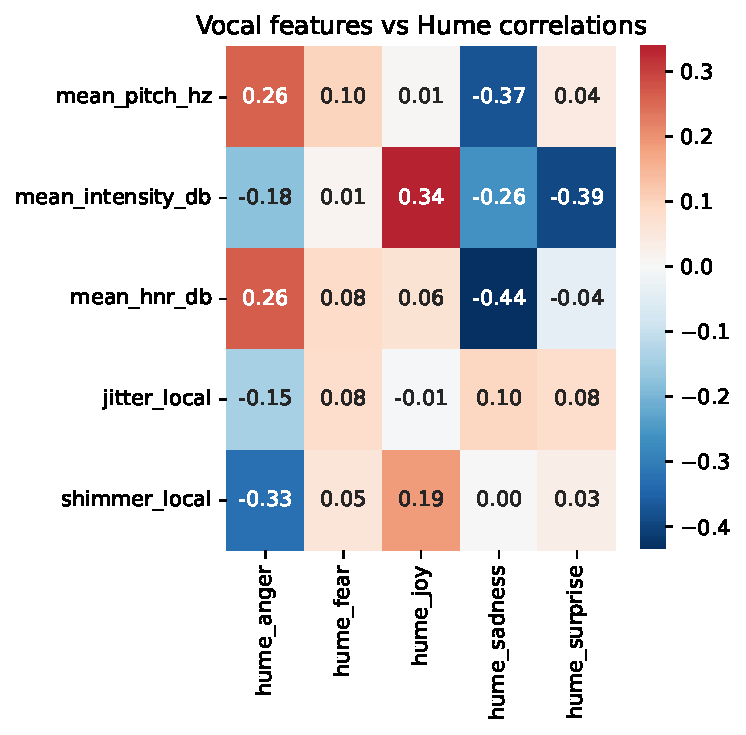
\includegraphics[width=0.6\textwidth]{png/results/rq1/vocal_features_vs_hume_correlations.pdf}
    \caption{Heatmap of correlation between vocal markers and Hume labels.}
    \label{fig:heatmap-voc-hume}
\end{figure}

Figure~\ref{fig:heatmap-voc-hume} demonstrates a heatmap of the Pearson correlation coefficients between selected vocal features and Hume AI emotion labels across all clips in the dataset. The results show generally weak correlations, with most values in the range of -0.4 and 0.3. 

\medskip
Key findings: 
\begin{itemize}
    \item Mean pitch (Hz) shows a moderate correlation with both anger (r = 0.26) and surprise (r = 0.04). This partially aligns with expectations from the previous research \autocite{Ekberg2023}, that showed elevated pitch was associated with high-arousal emotions such as anger and joy. 
    \item Mean Intensity (dB) has a positive correlation with joy (r = 0.34) and a negative correlation with sadness (r = -0.26) and surprise (r = -0.39). These results align with the referred research indicating that vocal intensity tends to increase with positive arousal states \autocite{Ekberg2023}. 
    \item Mean HNR has a slightly positive correlation with anger (r = 0.26), but shows weak correlations across all other emotions.
    \item Jitter and shimmer showed weak correlations, which may reflect that these features are subtle in spontaneous speech contexts compared to controlled or acted settings.  
\end{itemize}
Overall, the correlations with Hume suggest minor tendencies that reflect known vocal-emotion relationships, especially regarding pitch and intensity. The low degree of these correlations indicates that selected acoustic features alone did not strongly predict AI-detected emotions. 

\subsection{Correlation with Praat-Based Emotion Scores}

\begin{figure}[H]
    \centering
    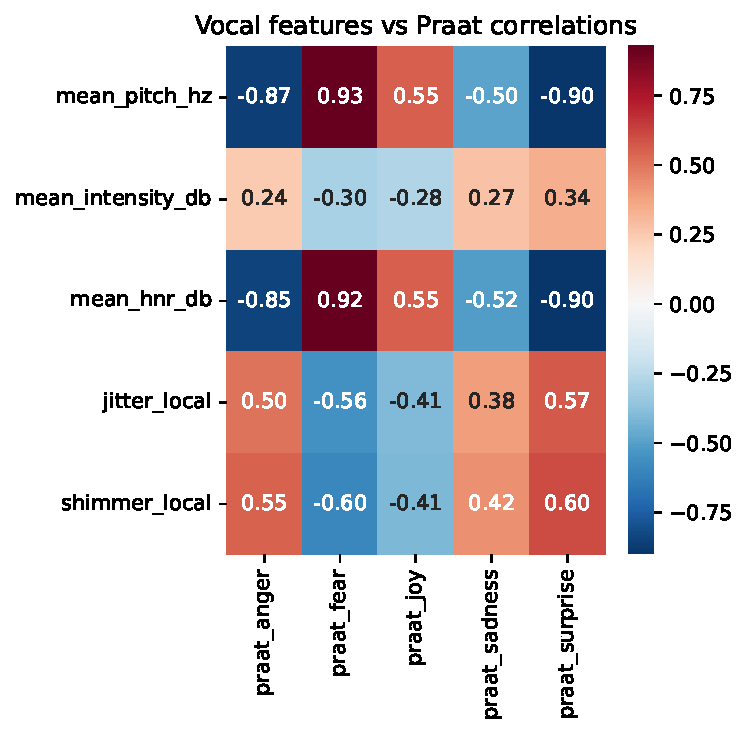
\includegraphics[width=0.6\textwidth]{png/results/rq1/vocal_features_vs_praat_correlations.pdf}
    \caption{Heatmap of correlation between vocal markers and custom emotion categorization.}
    \label{fig:heatmap-voc-praat}
\end{figure}
Figure~\ref{fig:heatmap-voc-praat} illustrates correlation between vocal features and the emotion scores obtained from the custom Praat-based categorization function. In contrast to the results for Hume, these correlations are notably higher. However, it shows patterns that are inconsistent with theoretical expectations. 
\medskip
Key findings: 
\begin{itemize}
    \item Mean pitch (Hz) shows very strong correlations (r = -0.87) with anger and fear (r = 0.93), which suggests that pitch strongly impacted the outcomes of the categorization. 
    \item Mean HNR (dB) revealed similar strong correlations as pitch, with high values for anger (r = -0.85) and fear (r = 0.92). 
    \item Jitter and shimmer display moderate to strong correlations as well, with varying directions for different emotions. 
\end{itemize}
The results suggest that the Praat-based function weighted some vocal features very heavily, especially pitch and HNR, resulting in inflated correlations that may be misleading. The absence of varying differences across the emotions suggest that the rule-based approach did not capture some expressions in spontaneous, interviewed, speech. 

\subsection{Limitations of the Custom Vocal Emotion Categorization Method}
To evaluate the performance of our custom emotion categorization function, which was developed based on vocal markers reported in the Swedish study \autocite{Ekberg2023}, we compared the emotion labels to the labels generated by Hume AI’s speech-based emotion recognition model. This comparison included both individual clip level and across the full dataset. 

However, the results revealed significant limitations in our approach. Regardless of the vocal input from our dataset, the categorization function consistently rendered near homogeneous emotion scores across all five emotions. This indicates that the function failed to capture emotional distinctions within spontaneous, conversational speech during interviews, regardless of theoretical relevance. 

Figure~\ref{fig:scatter_hume_praat} illustrates this issue across the full dataset, where the average scores assigned by our Praat-based categorization remain clustered around 0.2 across all emotions. Opposed to Hume that had greater variation through its labeling and reflects a more dynamic emotional detection.

\begin{figure}[H]
    \centering
    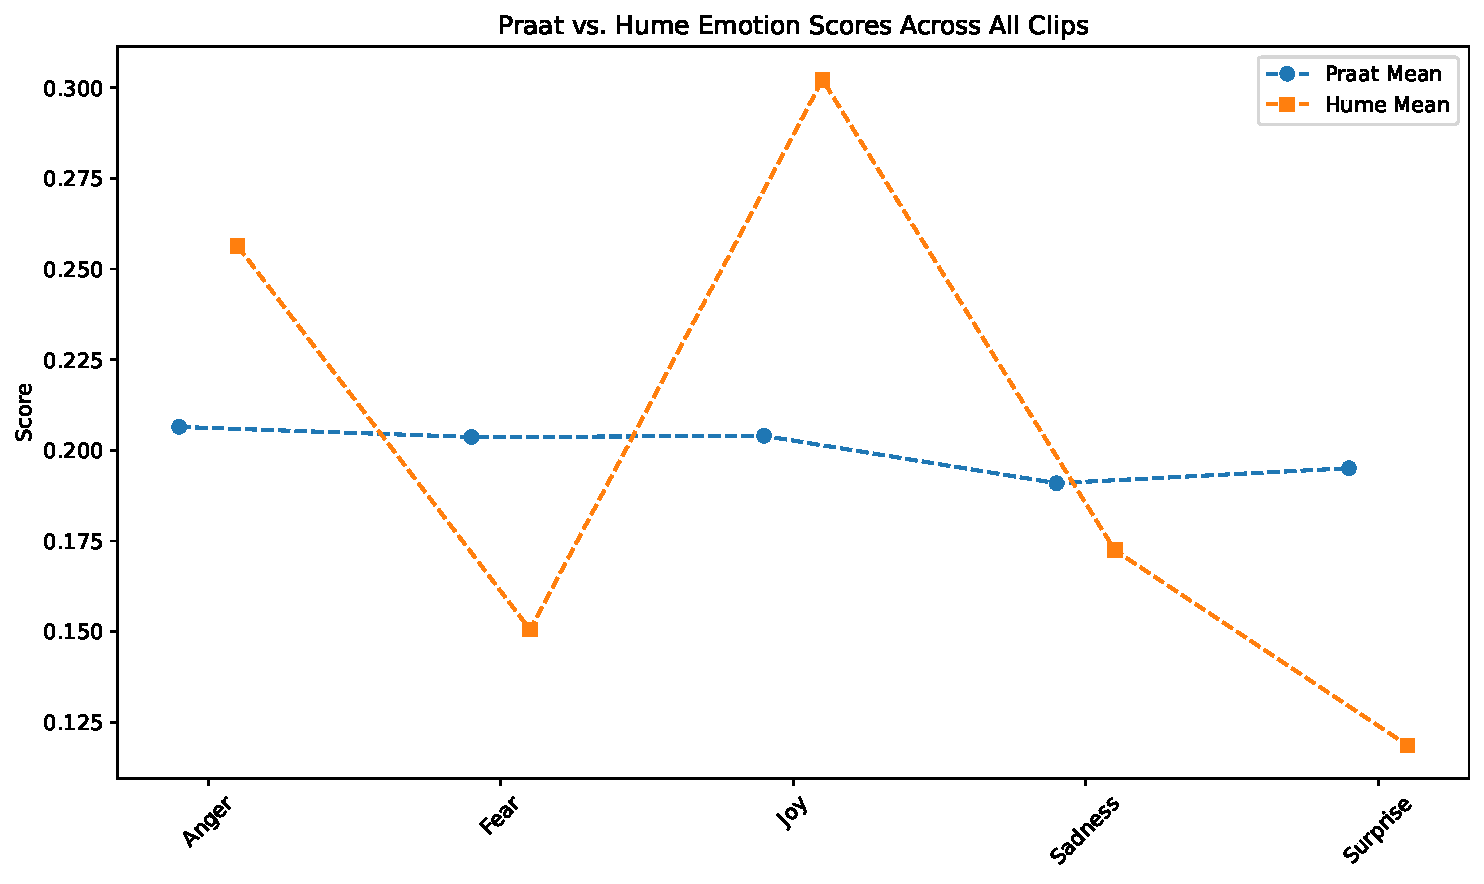
\includegraphics[width=0.7\textwidth]{png/results/rq1/praat_hume_all_clips_scatter.pdf}
    \caption{Average Score of vocal features-categorization and Hume labeling across all clips.}
    \label{fig:scatter_hume_praat}
\end{figure}

This is presented similarly in Figure Y, which presents a comparison for a single negative directed interview \texttt{id\_008\_neg}. In the same way as in Figure~\ref{fig:scatter_hume_praat}, the Praat-based scores are distributed very evenly across all emotions, while Hume assigns a higher probability to anger and lower for surprise,
with joy, sadness, and fear clustered more closely. Despite the fact that the score diversity between the Hume-labeled emotions are relatively moderate - approximately 0.10 between anger and sadness/joy, and around 0.15 between surprise and sadness/joy - the probabilities are still more diverse and provide a more interpretable output. The variability could be considered more reflective of potential emotional nuances in the interview. 

These findings demonstrate that our vocal feature-based categorization lacked sensitivity and adaptability when applied to our interview-based Swedish speech data. As a result, subsequent analyses focused on direct comparisons between raw vocal features and AI-predicted emotions, instead of relying on this flawed categorization method. 
\begin{figure}[H]
    \centering
    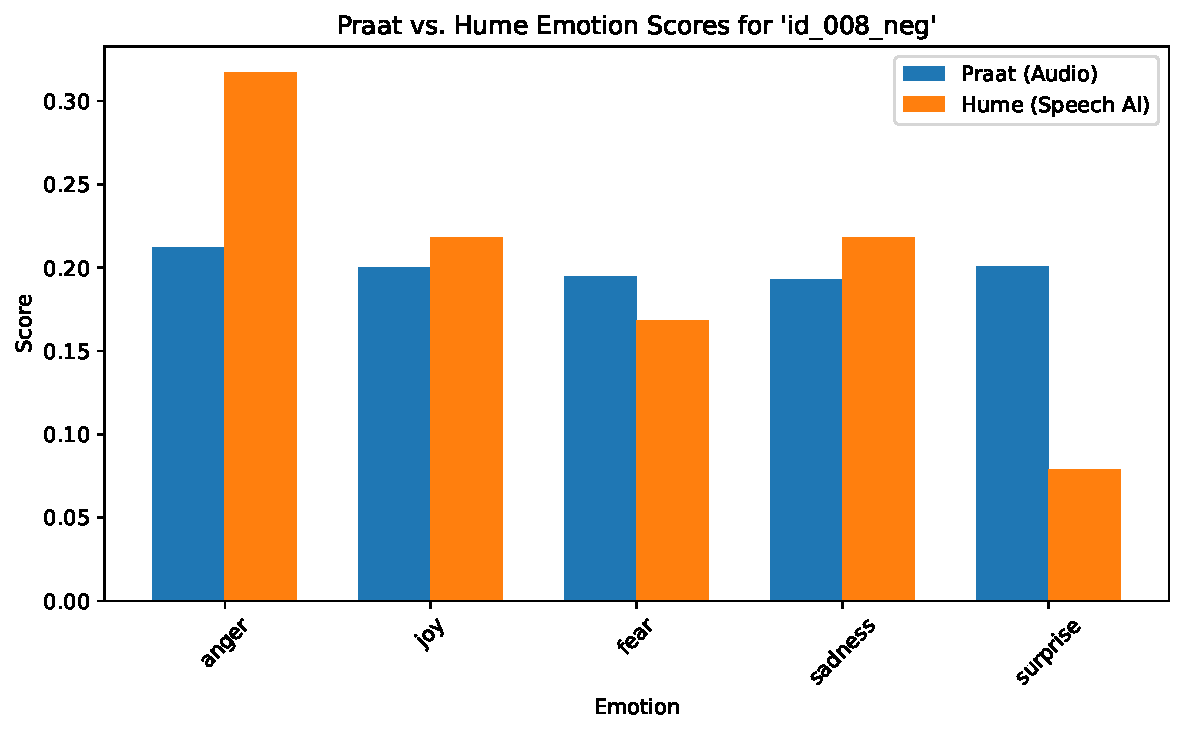
\includegraphics[width=0.7\textwidth]{png/results/rq1/id_008_neg_praat_hume_comparison.pdf}
    \caption{Vocal feature-categorization vs. Hume for single clip.}
    \label{fig:praat_hume_008}
\end{figure}

\subsection{ANOVA Summery of Vocal Features Across Emotions}
An ANOVA was implemented to further examine whether essential vocal features varied across AI-labeled emotions. This was conducted on pitch, intensity, HNR, jitter, and shimmer. The results are summarised in Table~\ref{tab:anova-rq1} and showed that none of the features showed statistically significant differences between the five Hume emotion categories (all p-values > 0.23). To confirm these findings, Tukey HSD tests were conducted and resulted in no pairwise comparisons between emotion labels with significant difference. 

\begin{table}[H]
    \centering
    \begin{tabular}{l|r|rrr}
    \multicolumn{1}{c|}{\textbf{Feature}} & \multicolumn{1}{c|}{\textbf{ANOVA p-value}} & \multicolumn{1}{c}{\textbf{Significant Differences}} &  &  \\ \cline{1-3}
   
    mean\_pitch\_hz                      & 0,4435                                     & No                                                   &  &  \\
    mean\_intensity\_db                  & 0,5793                                     & No                                                   &  &  \\
    mean\_hnr\_db                        & 0,2327                                     & No                                                   &  &  \\
    jitter\_local                        & 0,7797                                     & No                                                   &  &  \\
    shimmer\_local                       & 0,385                                      & No                                                   &  & 
    \end{tabular}
    \caption{ANOVA table for vocal features variance across emotions}
    \label{tab:anova-rq1}
\end{table}
These results imply that within our dataset of spontaneous speech during interviews, the average values of the acoustic features did not systematically vary according to AI-labeled emotions. This could indicate that emotional expression in conversations during interview circumstances is either: 
\begin{itemize}
    \item More subtle than in controlled studies.
    \item Features like pitch and intensity fluctuate instead of differing consistently at the audio clip level. 
    \item A deficient set of vocal features were extracted for these analyses. 
\end{itemize}
The lack of variance in these results does not align with findings in controlled settings \autocite{Ekberg2023}, where clear differences in vocal features were found between different emotional states. 

\subsection{Correlation Between Vocal Features and Hume AI Emotion Scores}
Considering the limitations that had been identified in our vocal feature-based emotion categorization function, subsequent analyses shifted focus towards examining direct correlation between raw acoustic features and AI-predicted emotions. Instead of applying predefined vocal emotion mappings to rely on, essential vocal markers have been investigated to obtain an understanding of how these correlate with Hume AI’s emotion scores across our dataset. 

\subsubsection{Composite Correlation Overview}
Figure~\ref{fig:composite} illustrates a composite correlation analysis, including Pearson correlation coefficients (r) between two acoustic features - pitch and intensity - and the given emotion categories that are filtered from Hume AI. Even if the correlations are generally moderate, certain patterns appear which aligns with previous findings in vocal emotion research. 
\begin{figure}[H]
    \centering 
    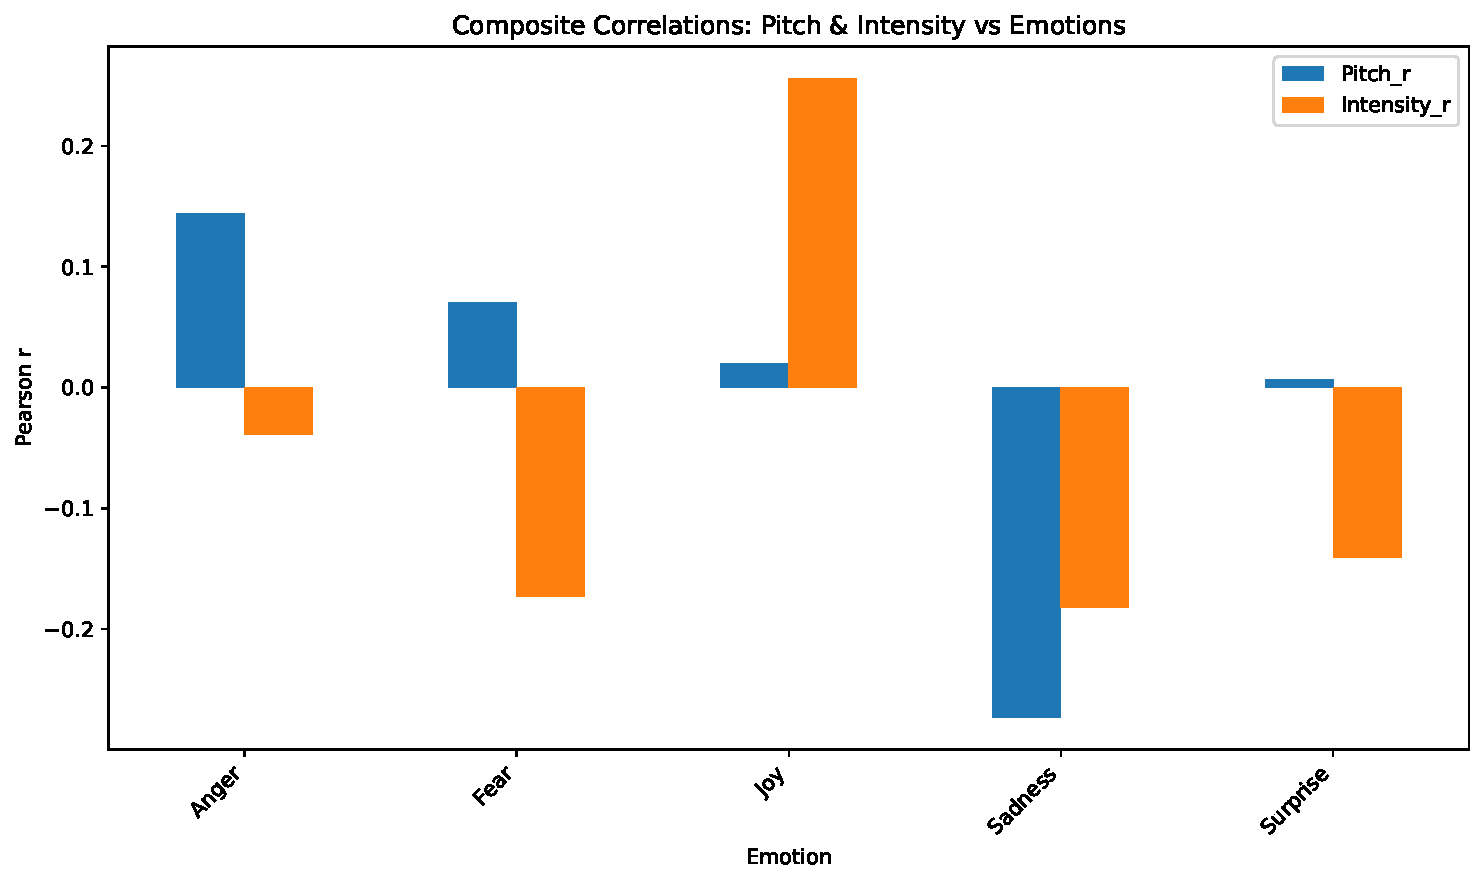
\includegraphics[width=0.6\textwidth]{png/results/rq1/composite_correlations.pdf}
    \caption{Composite correlation analysis}
    \label{fig:composite}
\end{figure}

Particularly intensity shows a positive correlation with joy, and suggests that higher vocal intensity tends to co-occur with AI detected happiness. In contrast, intensity shows a negative correlation with emotions such as sadness and fear, which is aligned with the expectations that these emotions are generally expressed with lower vocal energy. 

For pitch, a minor positive correlation is found in correlation with anger and fear, also reflecting expectations reported in prior research, where higher pitch is associated with heightened arousal states, for example anger. A negative correlation between pitch and sadness is shown, also supporting the prior findings where sadness is linked to lower pitch. 

However, the correlation strength is weak across all emotions, without values that indicate a strong linear association. This indicates, as our previous results, that single acoustic features like pitch and intensity alone are insufficient markers of emotional states when detected by speech emotion recognition systems, in the context of conversational, but interviewed, speech. 

\subsubsection{Supporting observations from individual clips}

For a more concrete illustration of the prior tendencies stated, two interview recordings were analyzed in detail. The purpose was to examine whether emotional shifts become more apparent when evaluating shorter time segments within individual speakers, compared to the weaker correlations observed at the dataset level.

In Figure~\ref{fig:pitch-4-pos} and \ref{fig:intensity-4-pos}, data is demonstrated from a positively directed interview \texttt{id\_004\_pos}, female, which shows that increases in pitch and intensity considerably often correlate with higher joy probabilities by Hume AI. While the correlation is not consistent throughout the recording, these moment-to-moment variations reflect the general expectation that higher vocal energy is associated with positive emotional expression. 

\begin{figure}[H]
    \centering
    \begin{subfigure}[b]{0.47\textwidth}
        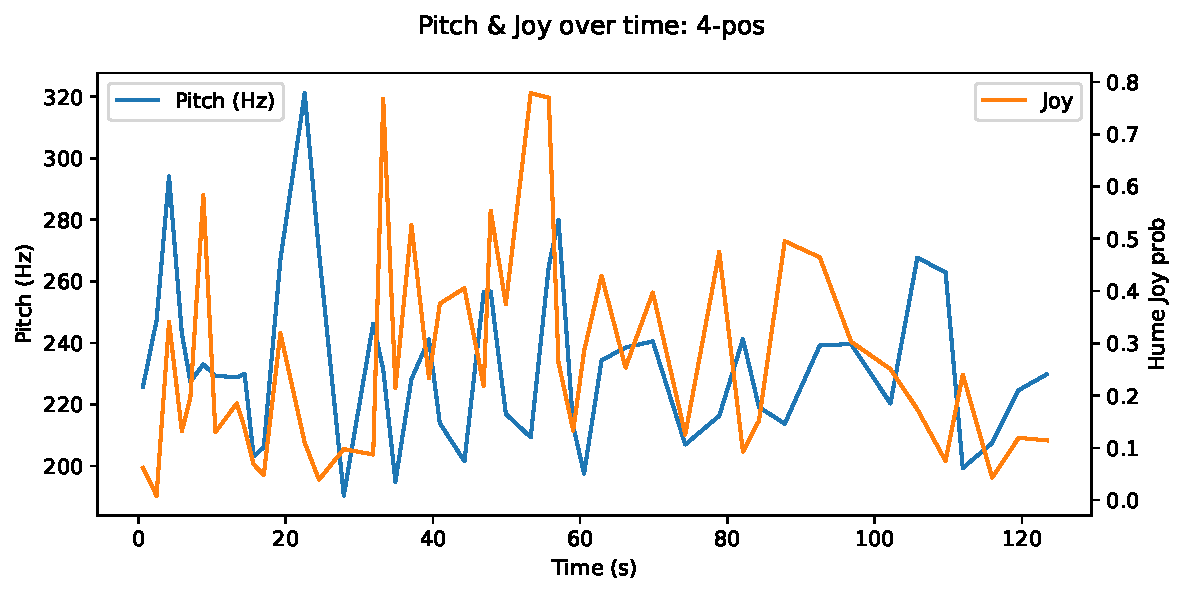
\includegraphics[width=\linewidth]{png/results/rq1/pitch_joy_4-pos.pdf}
        \caption{Pitch(Hz) and Hume label joy over time. Clip 4-pos}
        \label{fig:pitch-4-pos}
    \end{subfigure}
    \hspace{0.04\textwidth}
    \begin{subfigure}[b]{0.47\textwidth}
        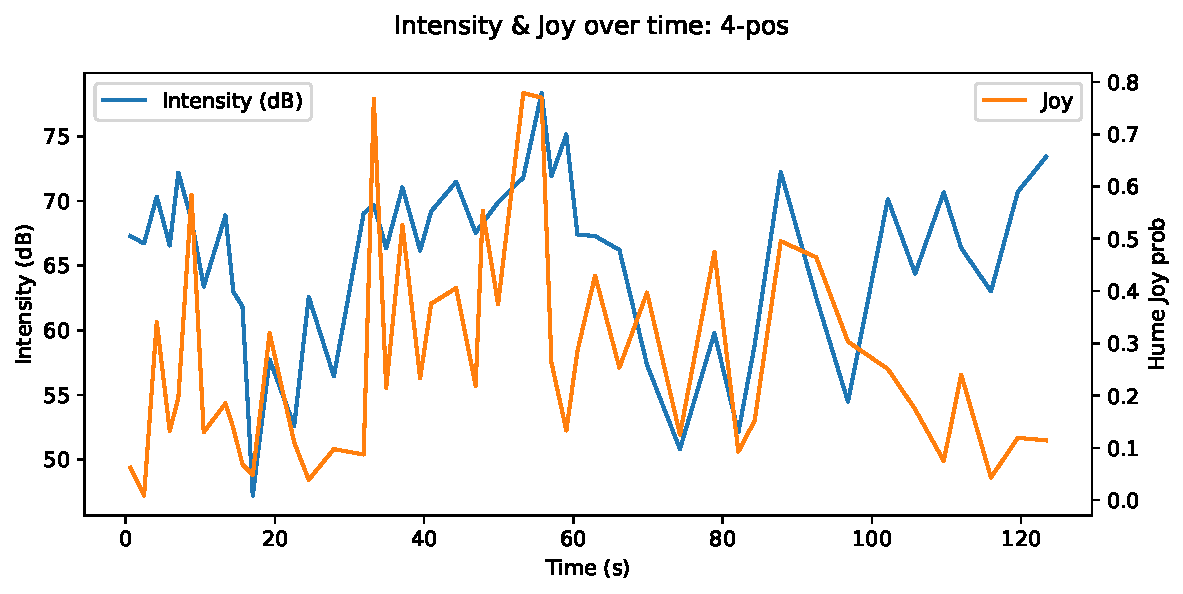
\includegraphics[width=\linewidth]{png/results/rq1/intensity_joy_4-pos.pdf}
        \caption{Intensity(dB) and Hume label joy over time. Clip 4-pos}
        \label{fig:intensity-4-pos}
    \end{subfigure}
\end{figure}

Similarly, Figure~\ref{fig:pitch-15-neg} and \ref{fig:intensity-15-neg} and \ref{fig:z-score-15} present data from a negatively directed interview \texttt{id\_015\_neg}, male. Here, clear peaks in pitch and intensity correspond with increased anger probabilities. These results are partly aligned with prior research on vocal markers of high-arousal negative emotions, such as raised pitch and loudness during expressed anger. 

\begin{figure}[H]
    \centering
    \begin{subfigure}[b]{0.47\textwidth}
        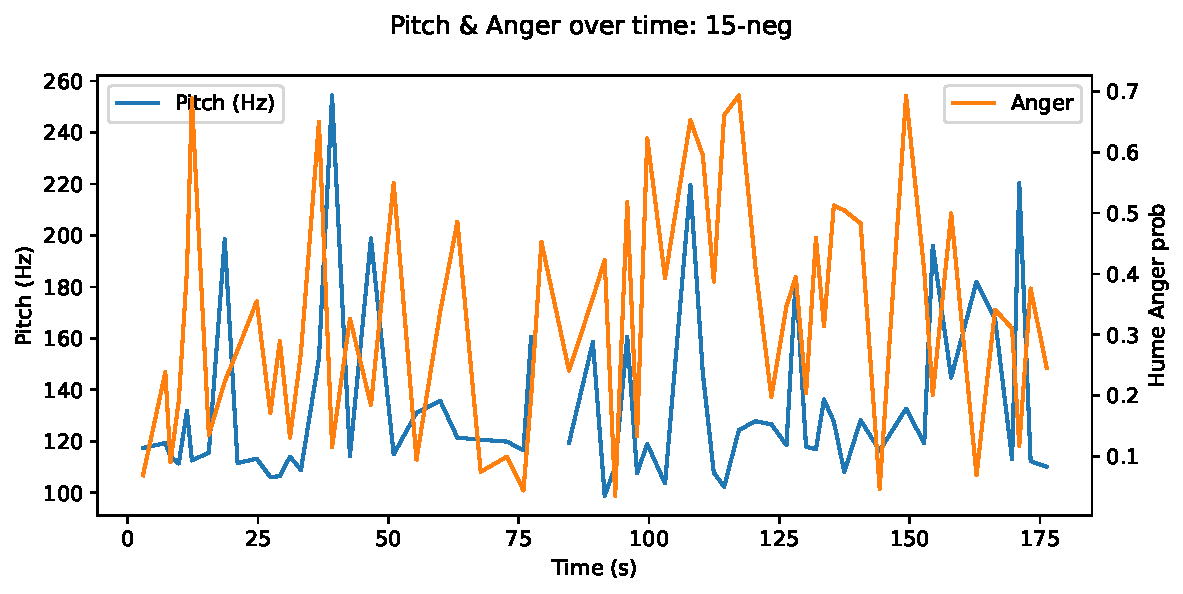
\includegraphics[width=\linewidth]{png/results/rq1/pitch_anger_15-neg.pdf}
        \caption{Pitch(Hz) and Hume label joy over time. Clip 15-neg}
        \label{fig:pitch-15-neg}
    \end{subfigure}
    \hspace{0.04\textwidth}
    \begin{subfigure}[b]{0.47\textwidth}
        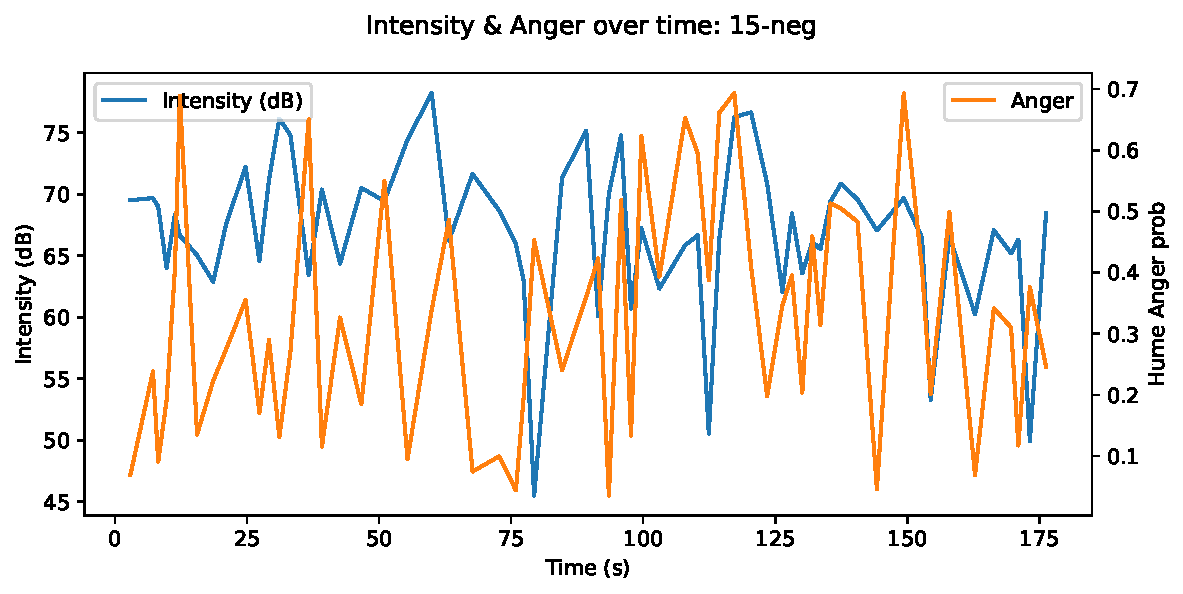
\includegraphics[width=\linewidth]{png/results/rq1/intensity_anger_15-neg.pdf}
        \caption{Intensity(dB) and Hume label joy over time. Clip 15-neg}
        \label{fig:intensity-15-neg}
    \end{subfigure}
\end{figure}

Additionally, Figure C illustrates z-score fluctuations of key vocal features for clip 13-neg. For this interview, several segments exceed +-1 standard deviation from the baseline, especially for pitch, intensity, and shimmer. These flagged moments align frequently with the emotion probabilities of Hume, which strengthens the link between vocal patterns and perceived emotional intensity. 

The z-score fluctuation diagram Figure \ref{fig:z-score-15} illustrates the segments further where vocal features significantly deviate from baseline levels, in patterns aligned with associated high-arousal negative emotions such as raised pitch and loudness. 

\begin{figure}[H]
    \centering 
    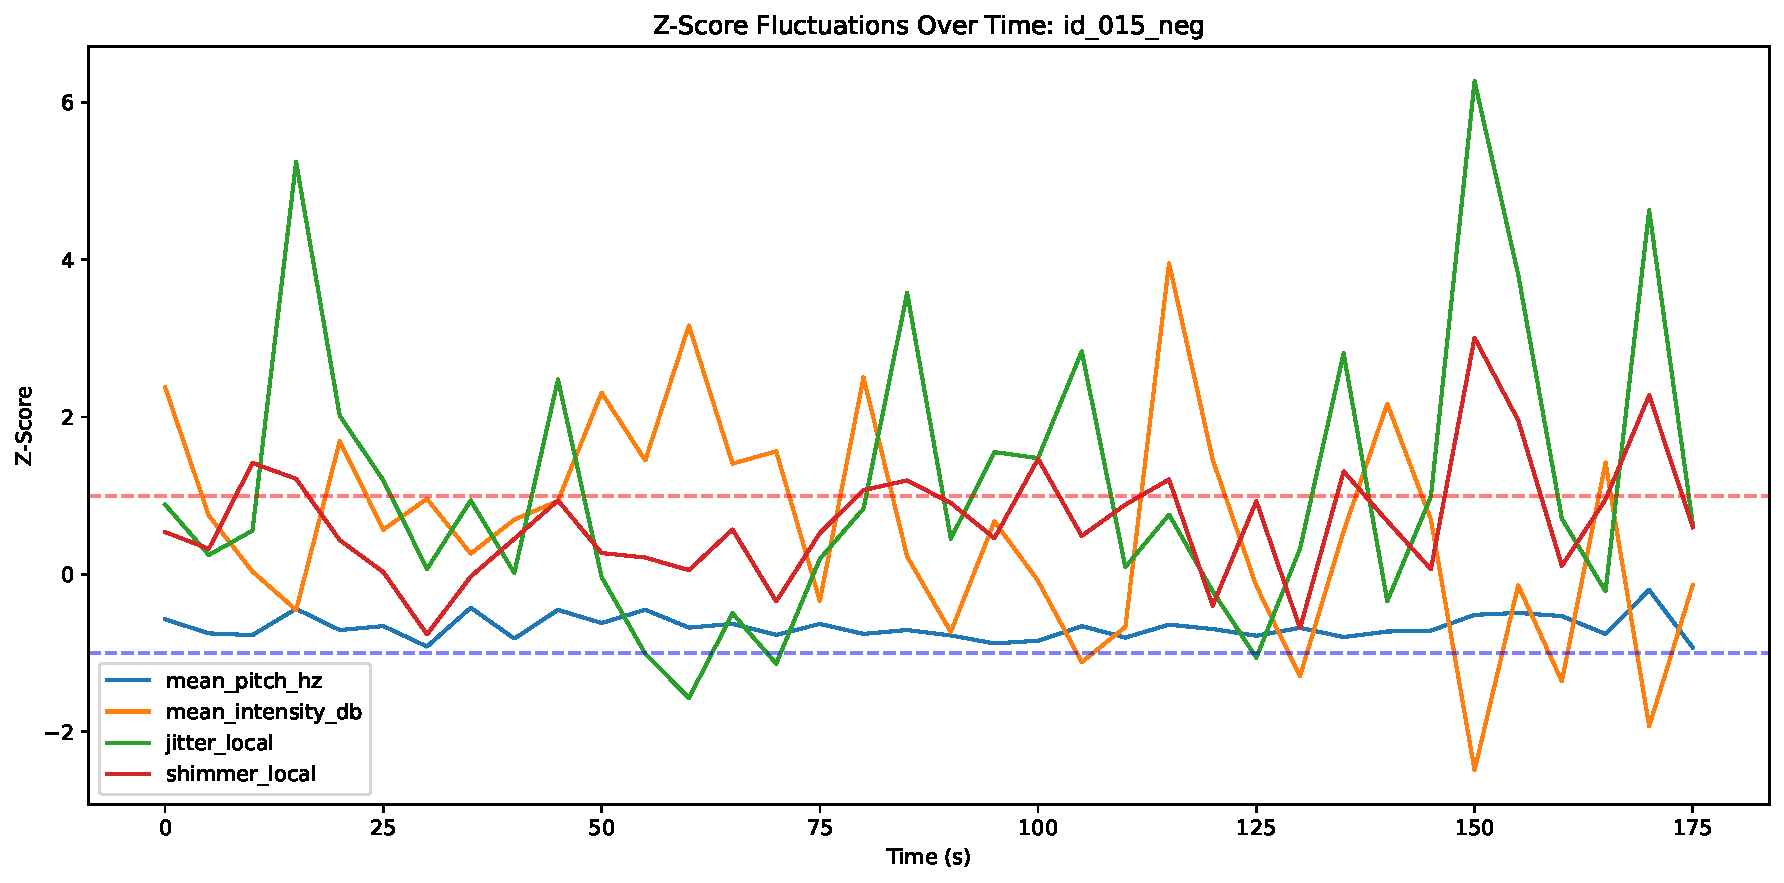
\includegraphics[width=0.7\textwidth]{png/results/rq1/zscore_fluctuations_id_015_neg.pdf}
    \caption{Z-score}
    \label{fig:z-score-15}
\end{figure}

\subsubsection{Summery}
This supports the idea that analyzing how vocal features change over time  can provide more meaningful insights into emotional expression in conversational, partly spontaneous speech during interviews compared to only using overall clip-level statistics.
\chapter{Discussion}
\label{sec:discussion}
\section{Result Discussion RQ1}

For the first research question, this thesis investigated how an AI model for speech recognition
compare to existing research on vocal markers. More specifically, the goal is to assess whether
the AI models align with the findings of the Swedish research on vocal markers done by \textcite{Ekberg2023}. 

The attempts to categorise emotions based the results on this Swedish study cannot be directly evaluated in terms of how accurate the function yielded emotion labels. Even if the standardised function had better recall against Hume, the divergences between the scores were minimal. 
The rule-based version got higher recall in addition of feature-based adjusting compared to Hume, which is not a ground truth, still beneficial for relative comparison. 
The improvement is aligned to prior research \autocites{Banse1996}{Ekberg2023}, minimising the extreme values for joy according to the wide acoustic markers while increasing the weight of pitch, which is stated to be the most prominent feature perceptually. 
Restricting anger to be required two of its studied characterises lead to slightly fewer recordings being top labelled as anger, which was added by the reason to separate anger from happiness. The final version presented some alignment between the top emotions, negative recordings yielded higher correlation where both models rated anger highest for six clips and sadness for two clips. More confusion occurred for the positive recordings. 
The interview setting is likely a contributor to this, where positive oriented questions can be answered with the same tone as negative evoked answers. 
Fear and surprise were rarely labelled by both methods, Hume distribution is presented in more detail for RQ2. 
However, even if the results yielded higher recall against Hume, it cannot be benchmarked that these alternations resulted in exactly the emotions that were expressed – a complex question to answer no matter what it is compared to, due to the nature of abstract perception of expressed emotional state, both internally and externally. When formulating the rule-based categorisation function, subjective opinions have an impact about fear and surprise rarely being expressed in the interviews overall, 
by the reason that the interviews were not designed to evoke these emotions which is complicated to recall in interview circumstances, especially for surprise. 

Comparison of vocal features against Hume’s emotions probability and our categorisation labelling demonstrates that the methods label emotions based on different data. Only sadness shows a similar vocal pattern between the sources, both negatively correlated with pitch and HNR, for other features, not as strong correlation similarities occur. 
No other emotion shows similarities, presumably by the reason that Hume has a much more advanced approach to recognising emotions than only using a few vocal features as indicators, as explained in Theoretical Framework~\ref{sec:vocal-markers}.  The fact that average values for a whole recording was used for these analyses, are most likely impacting the results due to low-expressed vs high-expressed segments even out.  
The subjective possible impact is a clear limitation as well as utilizing the Swedish research as a foundation for this categorisation since it is based on a small, acted dataset whereas this study analyses semi-structured interviews with spontaneous speech in conversational interview format. Limitations for the categorisation function also involves alternations that, even if motivated by prior research, might not yielding fully accurate results. 
Therefore, the remaining data analysis include Hume's probability and vocal features, not categorised manually.

To answer the research question, Time-to-Time analysis reveal what occurred for sadness in the comparison between vocal features and both emotion categorisation methods. Highest correlation values together with shifts for high-emotion occurrence with certain features resulted in sadness being most prominent predicted when pitch and HNR was lower, but also when intensity decreased. 
All three relationships are aligned to the Swedish research, where these acoustic markers have lower mean than other emotions. 
Fear was the second emotion with higher correlations, for example being predicted when pitch and HNR was raised, also according to the utilized research results. Joy had the highest intensity shift, that is stated in the research. However, anger had lower results for intensity which contrasts with expectations. 
When interpreting these results, it is important to acknowledge that the Swedish research do not specify how strongly the emotions are expressed, it is hard to define if anger is perceived as screaming or as a negative tone. 
Again, the nature of emotions is complex, and it is not possible to compose if the results are good or bad, which was not the purpose of this study. Conducting time segmented analyses generated additional insights that reduced the limitation with using mean values from the recordings, revealed by observing feature shifts. 


Despite that less than half of the feature-emotion group was significant, with most correlations being weak, certain patterns aligned with theoretical expectations was disclosed. The case examples provide a visualisation on both how certain vocal features align with Hume-predicted emotions, presenting similar patterns as prior research. It also shows how the fixed time-segments can have a negative impact on the correlation values, since Hume have clip varying time frames, the segments are not fully aligned.  
While correlations between AI-labelling and vocal markers are generally weak to moderate, it is important to acknowledge that Hume emotion scores should not be perceived as perfect estimates of true emotional states, even if it probably results in reasonable predictions. 
These analysed recordings consist of spontaneous and conversational speech which likely do not involve as strong emotional expressions as acted datasets, with tendency of more subtle and reduced level of vocal features. The simplicity regarding the number of applied vocal markers in contrast to the emotion-trained AI model reaching beyond the use of single acoustic features is a certain reason that this study should be interpreted as explanatory and not to benchmark the general efficiency of emotion recognition in Swedish speech.    

The wide acoustic spread for certain emotions, as anger and joy, presented in both \autocites{Banse1996}{Ekberg2023} and was prominent when adjusting the rule-based emotion categorisation where alternations had to be included to seperate them from each other. 
This imply that vocal-marker theory can be limited in conversational context and the intention of the speaker, such as sarcasm and genuine versus polite emotions. 

Certain vocal patterns do in fact recognize expressed emotions, as we as humans can interpret certain emotions in others through their speech, algorithms and technology can do the same, at least to some extent. 
Even if some Hume-labelled emotions align with research on acoustic markers, more than these features are utilized to recognise emotions with AI. The fact that some alignment arise between the Swedish research and Hume AI, 
suggests that the language does not necessary have an overly negative impact, yet our results are not comprehensive enough to confirm this. 

\section{Result Discussion RQ2}
For the second research question in this thesis, the aim was to investigate the similarities and differences between the two AI models Hume AI, a speech-based model, and NLP Cloud, a text-based model. This was measured when labelling five different emotions in semi-structured interviews.

\label{subsec:RQ2interpretation}
In the comparison between the speech-based emotion recognition model and the text-based emotion recognition model, the system overall seemed to show some levels of agreement for certain emotions. Using both descriptive statistics and visual analyses to calculate the differences, an overall comparison of both ai systems showed that the mean emotion scores differ across the two models.

The average difference in the emotion presented in table~\ref{tab:rq3_emotion-stats-combined} scores for all recordings showed values indicating that Hume AI obtained higher scores for the emotions anger and fear, while NLP Cloud proved to show higher scores for joy, sadness and surprise. Despite these findings, the score for sadness and surprise were sufficiently low, suggesting that the models were substantially aligned on specifically those emotions, although is important to note that this table shows the average for all recordings. Taking the average of both the positive and negative recordings likely resulted in the opposing emotion values suppressing each other, leading to a more neutral score.

In figure~\ref{fig:rq2_sent_grouped_bar}, the results of the entire dataset divided between the positive and negative recordings were presented. These results showed NLP Cloud having a significantly higher mean emotion score for joy and a slightly higher score for surprise in the positive recordings. In the negative recordings, NLP Cloud had a higher score for anger and sadness. 

Hume on the other hand, showed a significantly higher emotion score for anger, and a somewhat higher score for sadness and fear in the positive recordings. For the negative recordings, only joy showed a very significantly higher score compared to NLP Cloud, whereas fear and surprise showed to be somewhat aligned between the two models. Joy being highly scored for Hume AI in the negative recordings may be due to some signals being misinterpreted when speaking of negative topics, for example some participants may have talked about the negative topics in an ironic tone or with sarcasm or expressed nervous laughter, which would be hard for a speech-based model to differentiate and pick up on without the textual context.
Another possible explanation may be due to pitch variations. Earlier research found that prosodic features like pitch are informative for arousal detection (källa****Soleymani2017****). Pitch is one of the key features for emotion recognition in audio and it is possible participants of the interviews may have spoken with a high pitch even if not using a very descriptive language. Hume AI could have interpreted a high pitch as emotional intensity, possibly explaining the high score of joy in the negative recordings and the high score of anger in the positive recordings.

Joy being highly scored by NLP Cloud in the positive recordings indicates that joy may not have been as easily identified in speech-based emotion analysis, as the textual context may have conveyed a more positive tone from the text than what appeared in the voice. In contrast, anger and fear appeared to have been more effectively captured by the speech-based emotion detection in the positive clips, possibly suggesting that someone might sound angry or fearful even though they may not be experiencing these emotions in the moment. This is further backed up by earlier research stating specific words like “amazing” holds more intensity for emotions than other words like “leaves” (källa****chau 2024****). The participants in the interviews may have used very descriptive language when describing positive experiences, which may be a reason for the high score for joy by NLP Cloud.


Based on the Pearson correlation analysis in table~\ref{tab:corr_all}, showing the association between the text-based and speech-based emotion recognition models for all recordings, the strongest alignments were shown for Joy (r = 0.521) and anger (r = 0.466). Joy and anger also showed statistically significant p-values, where joy had a p-value of 0.002, and anger had a p-value of 0.007. No further strong correlations or statistically significant p-values were found in the other emotions.

Several factors may account for this result. For example, joy and anger are distinct emotions, while sadness, fear and surprise may likely involve more subtle cues and contextual factors. Being more complex to detect may have contributed to the lower consistency across the two models for these specific emotions. Research have found that acted speech involves a stronger degree of intensity than spontaneous speech, which makes it more difficult to recognize emotions in this format (källa****Chakr 2016****). With spontaneous speech from interviews was used in this study, it’s very possible the models failed to detect the low-intensity emotions.

For the positive recordings only, there were two emotion showing significant correlations between the two models, joy (r = 0.160, p = 0.568) and sadness (r = 0.549, 0.035), whereas for the negative recordings the only emotion that showed a significant correlation was joy (r = 0.556, p = 0.020).

These results suggests that joy is the easiest emotion to detect for the models regardless of the context, and that anger, fear and surprise may be too complex to detect, although there are several possible reasons as to why they have low or inconsistent correlations. The way that the interviews are set up and the fact that the participants of the interviews talk about situations and feelings they have lived through in the past, may have resulted in emotions being expressed in a subdued way. Talking about a time where you felt fear or surprise might not be translated as strongly when time has passed, as it would in the moment when the emotions were felt. It is possible the interviewees did not feel or express strong emotions when speaking about different situations, and as neutral emotions have been found harder to detect according to earlier research (källa****cao 2015****), it is possible some emotions have remained undetected or incorrectly detected.

With this in mind, the lack of correlations for more complex emotions suggest that the interview format may have been insufficient to draw out more nuanced emotional responses. Alternatively, the AI models used may have some limitations in detecting subtle emotions.


For the full dataset, paired t-tests showed no significant differences for the mean score of the emotions across the dataset for all emotions except fear. Although the correlation between Hume AI and NLP Cloud showed non-significant scores for fear, the t-test indicated that while the systems do not align on detecting patterns for fear, Hume AI consistently rates the fear higher than NLP Cloud. Possible explanations for this result may reflect the differences in how emotions are conveyed and detected in the different models, whereas Hume AI possibly could have captured the more subtle vocal indicators that might not have been as easily expressed or detected in text.

In examining the t-tests for the positive oriented interviews in comparison to the negative oriented interviews, notable findings emerged.

For the positive interviews, significant differences between Hume AI and NLP Cloud were found for all emotions with the exception of surprise, where Hume consistently detected higher levels of anger, sadness and fear. NLP on the other hand overestimated joy significantly in comparison to Hume. 
This may be explained by the complexity of emotions and emotional expression. In the positive interviews, the participants discussed joyful topics, and while this may have been detected for the text-based emotion recognition, the vocal tone could reveal more subtle cues in the tone, rhythm and pitch. For the positive interviews, the participants may have had a lower and more neutral tone and pitch than an actor acting out happiness, which could be one explanation for this result, which also can be explained by earlier research stating neutrality makes detection of emotions more difficult  (källa****cao 2015****).

For the negative interviews, significant differences were only identified for joy and sadness, where Hume rated joy with a higher score, and NLP rated sadness higher. This indicates a better alignment for the different models for the analyses made for the negatively oriented interviews.

Possible explanations for these results are that people participating in the interviews may have used overly positive language out of politeness, even if the content of the words may have been negative, which would explain why Hume AI detected joy from negative oriented interviews.


\section{Result Discussion RQ3}
For the third and final research question, the objective was to assess how the AI generated emotion labels obtained through the speech-based and text-based emotion recognition would compare to the self-reported emotions provided by the interviewees.

In examining the alignment with the speech-based emotion labels from Hume AI and the text-based emotion labels from NLP Cloud with the self-assessed emotion scores, insightful findings revealed some levels of alignment dependent on both the model and emotion.

Figure~\ref{fig:comp-bar-rq3-all} builds on figure~\ref{fig:rq2_sent_grouped_bar}, discussed for RQ2. Presenting mean emotion scores for Hume AI and NLP Cloud, figure~\ref{fig:comp-bar-rq3-all} also introduced the self-assessed emotion scores.
Key differences were found between the models in comparison to the scores obtained from the interviewees, as NLP Cloud rated joy much higher than both the other modalities. As earlier discussed in section~\ref{subsec:RQ2interpretation}, this could still be explained by the spontaneous interview format in a calm setting, as this format may not encourage expressively conveying emotions, leading to the model interpreting textual language as joyful even though the tone may have been more neutral.
Suprise presented almost identical values for the self-assessed scores in comparison to NLP Cloud, although for all other emotions (anger, sadness and fear) the participants of the interviews rated their emotions almost an average between the two models, with the scores not being quite as high as Hume AI, and not as low as NLP Cloud. In the case of Hume AI estimating anger substantially higher than NLP Cloud and somewhat higher than the interviewees themselves, there might have been misinterpreted signs of anger coming from pitch and intensity during the interviews. These results suggest that the only emotion detected somewhat similarly here compared to the self-assessed scores, was surprise, whereas the self-scores landed on a middle ground between the two models for all other emotions in the positive oriented interviews.
Higher ratings of anger by NLP Cloud compared to the two other sources was likely due to the context of negative wording in the negative interviews forwarding the emotions more than was both felt by the participants and detected trough the voice.
NLP Cloud scored substantially closer scores to the self-assessed emotion scores for joy and sadness compared to Hume AI, suggesting the context of the words matched the emotions in the interviews better which indicates that the text-based model might have been better at capturing emotions from the vocal recordings. Hume may not have picked up vocal cues in the same capacity, likely due to the low expressions and more neutral speech during the interviews. This further reflects a limitation in emotion recognition from spontaneous speech, which also has been highlighted in earlier research. Research done by \textcite{Cao2015}, found even advanced ranking-based classifiers which had outperformed traditional models, to struggle with neutrality in spontaneous speech \autocite{Cao2015}.
Further analysis for the negative clips showed Hume AI rated the emotion joy extremely high in comparison to the two other modalities. This further confirms what was earlier explained in the discussion for RQ2 ~\ref{subsec:RQ2interpretation}, that Hume AI may have incorrectly interpreted certain vocal cues as joy, for example nervous laughter or sarcasm, which could be difficult for a speech-based AI to recognize.

Overall for the sentiment-based comparisons, the negative recordings showed a better alignment for all three modalities. For both the positive and negatively oriented recordings, the two models performed better for some emotions as the text-based AI NLP Cloud seemingly captured the context for each interview more effectively for some emotions than the speech-based model and vice versa. This underscores the limitation of relying exclusively on either speech-based or text-based emotion recognition, as the different models capture different emotions with varying success. Using both models in comparison to the self-assessed scores gives a wider understanding of the performance for the text-based versus speech-based emotion recognition model and their different strengths and weaknesses. This aligns with earlier research which also have concluded that using more than one approach results in a better performance than only relying on an individual source \autocite{Cao2015}.

When examining the positive recordings and the negative recordings individually for the correlation analysis for Hume AI, no significant correlations were found for any emotions, although the positive recordings showed moderate positive trends for anger and joy. These emotions did not reach any significant correlations, but moderate r-values suggests a possible relationship that may be of interest to explore in the future with a lager dataset or different methods, as the lack of statistically significant correlations indicated that the emotions captured in the interviews do not align closely with those in Hume AI. 
For the correlation analyses for NLP Cloud, surprise was poorly detected with low correlations, suggesting the model struggled with the interpretation of the emotion surprise, possibly as a consequence of the complexity of the emotion and once again the nature of the interview format.

While NLP Cloud showed stronger correlations with the self-reported emotions overall compared to the Hume AI model, results showed that the model performs inconsistently across the different contexts (negative and positive), suggesting that a more consistent recognition of emotions may demand more modalities for better accuracy. These results also point to the fact that surprise remains a complex emotion with more challenges to capture from the data used in this study, although there are additional reasons as to this challenge. In the self-evaluation segment of the interviews, multiple participants expressed certain confusion regarding the assessment of the emotion surprise. A large part of the interviews consisted of describing past emotional experiences which may have reduced the intensity of surprise. Typically, surprise is expressed as an immediate reaction to unexpected events and it’s unlikely that the interviewees are able to genuinely experience the same surprise felt in the original moment of the memory. This provides a possible explanation for why both AI models overall detected low levels of surprise, while an acted dataset could present higher correlations for this emotion. As stated in earlier research, acted speech is an amplification of emotions and spontaneous speech may lack the level of intensity to be distinguished from different emotions \autocite{Chakraborty2016}.

For the statistical analysis and effect sizes showed to be consistent with earlier findings, further giving grounds to this discussion. 
The full dataset showed Hume to have a moderate tendency for overestimation of the emotion anger in comparison to what the participants of the interviews had reported themselves, which remains true for the positive recordings where anger was very highly detected by Hume. As Hume also tends to underestimate surprise compared to the self-assessed scores, it is further confirmed that surprise is a difficult and complex emotion to detect. This validates conclusions from earlier research stating that neutrality is difficult for a model to deal with \autocite{Cao2015}. It is possible the neutrality of the speech often coming across in a spontaneous interview format may have been one of the reasons as to why emotions like surprise were detected at low levels. Hume AI as a speech-based emotion recognition model may not be capable of detecting subtle emotions and appears to struggle without the textual context as some vocal cues seems to have been misinterpreted.
No significant differences were found for NLP Cloud in the negative context, which further confirmed a closer alignment for NLP Cloud and the self-assessed scores in the negative contexts as earlier discussed in this chapter.
In the cases of where the alignment for the models and self-assessed scores did not align as well, further explanations can be drawn from earlier research stating sentiment do not inevitably display themselves in expressions or behaviors \autocite{Soleymani2017}. In many cases both Hume AI or NLP Cloud overestimated or underestimated scores compared to the self-assessed values, likely because of vocal expressions not always aligning with the internal affective states as sentiment is not always fully articulated.

\section{Method Discussion}
\subsection{RQ1 Methodological Considerations}
To answer RQ1, the methodological approach involved analysis of emotional expression for
vocal markers in Swedish speech in comparison to AI based emotion recognition models. The
idea was to analyse emotions in a clip in its entirety and find correlations, which had some
differing results, but it proved to be a notable strength to execute the analysis on a segment
level to capture emotional fluctuations in a more dynamic way. While this offers another
another perspective, this approach introduced challenges of its own in having some inconsistent
emotions not aligning completely across the segments. Output from Hume is pre-segmented with frequency variation of 1-4 seconds, single clip dependent. Vocal features were segmented into 2.5 second timeframes used for all clips, leading to divergencies in segment length. For more accurate results, it should have been adjusted separately for each clip before segmented analysis. The methodological approach for the RQ1 was partially fulfilled by identifying some vocal fluctuations in emotions, while also revealing challenges in both segment-level and average values. Further insights could have been provided with utilizing the rule-based functionality for emotion grouping segment wise as well, to find if grouped features could provide higher correlation results for Hume labelling and acoustic markers. 

Comparing the results with the prior study on Swedish vocal markers indicate some similarities and patterns providing valuable information to this study, even if several correlations and patterns remain weak. Mainly focusing on this study as reference may create bias, by the reason that there is vastly limited prior research on Swedish in this field. Additionally, this study employed a larger number of vocal features than extracted for these results. The three frequency formants were included in both categorisation functions yet excluded in the overall data analysis. Beyond these, the Swedish study included 14 additional features, some of these were not possible to extract with Praat Parselmouth and therefore excluded. Voiced- and unvoiced length were not relevant for this study since the recordings were edited, including deleting some silent moments. Not including the full set of features is a clear limitation for the results. [ADD INSIGHTS ABOUT THESE VOCAL MARKERS FROM STUDY HERE AND WHAT THEY COULD HAVE PROVIDED]. The data collection used in this study consists of interviews capturing spontaneous speech, contrasting the referred Swedish study based on pre-defined sentences, repeated by four actors. With 15 participants, the dataset for this study resulted in a total of 30 recordings across a diverse group of participants consisting of men and women with ages ranging from the 23-78. The spontaneous speech and large variety of interview questions combined with dataset size may indicate some limitations for the result. During the data analysis it was found that pitch and HNR are significantly diverged for male and females [APPENDIX]. This has most likely impacted the results for all analyses conducted on the full dataset, by the reason that these features even out by the other gender and may create a normalised average even if it would be distinct if analysed separately. 
Given that the dataset for this research consisted of interviews capturing spontaneous speech, a broader range of vocal features might have contributed to the detection of the complex vocal patterns and given a more
nuanced understanding of the correlations for emotion recognition in the Swedish language. While the selected vocal markings chosen for this study gave some insight into addressing RQ1, expanding the set of features could have helped address RQ1 more comprehensively.


\medskip
\subsubsection{ALL RQ } 
The interviews were designed to provoke one positive and one negative emotion, yet not directly oriented towards one of the three negatively oriented emotions. This structure was motivated by allowing the participants to talk freely about a subject they related to and felt comfortable to discuss. During the self-report after each interview, several participants raised confusion about how to interpret and rate surprise. This emotion showed most inconsistency throughout all research questions and was not aimed to be induced through the interviews. By reducing this study to only focus on one positive and one negative emotion, both for interview design and in data analysis, a more comprehensive analyse of only these emotions could be conducted to yield a narrower, yet deeper analysis of two focus emotions. On the other hand, patterns of vocal features for certain Hume-labelled emotions were benefited by enable comparison with all emotions used in the Swedish study. 

Hume AI was one of the models used and provided some advantages such as avoiding manual
labeling and being pre-trained, although the Hume AI emotion scores had to be normalized and
the emotions were filtered to use only the specific five emotions necessary for the comparisons
in this research, which may have had some limitations on the model’s capacity. Along with
working well for the research’s purpose, the model has some downsides. For example, there is
limited publicly available information about functions of the model, making it difficult to fully
assess possible limitations and biases. Despite these limitations, Hume AI contributed with valuable insights in answering RQ1.

Comparing our interview-based result with a larger and more controlled dataset with acted emotions could possibly have validated some observed patterns or strengthened the opposite whereas acted speech is expressed explicitly different from speech in real-world similar contexts. 

\subsection{RQ2 and RQ3 Methodological Considerations}
The methodological approach to address RQ2 combines analysis of transcribed text in emotion recognition using NLP Cloud in order to assess the emotional content of speech transcripts in relation to speech-based AI models.

In addressing RQ3, the approach was to compare self-reported emotions with the AI-generated labels from both speech and text-based models to analyze potential alignments.
This is a multi-modal approach with several methodological considerations, but also some methodological strengths.

The vocal recordings were transcribed and analyzed with the text-based emotion recognition tool NLP Cloud and self-assessments of emotions were collected after each interview, allowing a comparison between speech-based AI, text-based AI and self-assessment scores given by the participants in the interviews. 
The use of three different methods resulted in triangulation, which increased the flexibility and credibility in the findings. In addition to this, the usage of pre-trained AI models ensured consistent processing. However, some information loss was expected for the transcript text analyzed in NLP Cloud. When the model takes in what is said rather than how it is said, many important emotional cues such as intensity or pitch get lost. This could possibly have led to some emotions being misinterpreted or not catching the full complexity of the emotions expressed, based on only the text-based analysis.

While NLP Cloud contributed in addressing RQ2, some limitations in loss of prosodic information may have reduced the full emotional understanding.
The self-reported emotions introduced a valuable reference point for this research. Some agreement was found between the AI models and self-reported emotions, but some of the self-assessed scores may also have been slightly exaggerated. The emotional memories and personal interpretations of emotions by participants can have influenced the self-assessed emotion scores.
While the self-reported emotion scores have some limitations which likely contributed to some variability in the analyses, they helped valuably address RQ3.

The complexity of emotion detection across different modalities is highlighted by the AI models being able to capture some emotions in a quite robust way while struggling more with others. The few emotional categories used for this research may have limited the emotion recognition, where an implementation of more emotions and features possibly could have captured the emotions in a better way.

All methods used in answering RQ2 and RQ3 provided valuable information and findings, however the research could have benefited from an expansion of the emotion categories to help identify emotions in a more accurate and complex way.

\subsection{Summary of Methodological Considerations}
To address all research questions, this study utilized a multi-method approach combining speech-based and text-based emotion recognition with self-reported emotion scores of the participants from the interviews. 

Although all methods contributed with important findings and significant insights into emotional expression in Swedish speech, a number of limitations emerged.

While the triangulation of speech, text and self-assessment scores contributed to the strength and credibility of the findings, size of dataset, model transparency and other limitations such as variabilities and inconsistency in having spontaneous interviews may have impacted the effectiveness of the findings. Although highlighting some areas for improvement for future studies, the methods chosen for this research overall contributed to answering the research questions in a comprehensive manner.

\chapter{Conclusion}
\label{sec:conclusion}
\section{Summary of Key Findings and Answering Research Questions}
\label{sec:con-key-findings}
Based on the findings presented in chapter 4, the following key findings and answers to the research questions were found.

In the first research question, the aim was to compare the vocal features from speech recordings gathered from interviews to see whether or not they correlate with AI-based emotion detection from the model Hume AI. Existing research on vocal markers in Swedish speech was used for better comparison.
Here, the results showed some alignments between AI-based emotion recognition models with the existing research on vocal markers in Swedish language. Many correlations were weak or moderate and the results showed some limitations, for example. the nature of spontaneous speech involved in interviews presented challenges for some of the emotions, while other emotions proved to be more relevant indicators of emotional states. The results revealed that Hume AI showed promise with the contextual awareness and the flexibility of the model. 
In this research question, important insight was also given through the segment level analyses which presented the fluctuations in the emotions better than average clip analyses.

For the second research question, where the purpose was to investigate if emotions from textual content of speech, transcribed and analysed with the AI model NLP Cloud could be understood through comparisons made with the speech based AI model, Hume AI. Here, some agreements were found between the AI models Hume AI and NLP Cloud, for some emotions more than others. Joy and anger showed better alignment whereas fear and surprise did not align as much. The overall cause for this most likely being the complex nature of some emotions where the cues may not be as pronounced.

For the third and last research question, the comparisons between the AI models Hume AI and NLP Cloud and self-assessed emotion scores from the interviews were investigated. These results showed there were some alignments between the models and self-assessed scores, though these alignments were stronger with NLP Cloud than with Hume AI.
This gave insight into the fact that although some alignments were stronger with NLP Cloud than others, a multimodal approach that integrates several sources results in better detection of emotions, where only relying on either Hume or NLP Cloud would not give as much insight in the results.

Overall, the findings in this research provided answers to all research questions, contributing to a deeper understanding of emotion recognition in the Swedish language.
\section{Contribution to the Field}
\label{sec:con-contribution}
This thesis contributes to the vocal and linguistic aspect of the growing fields affective computing and natural language processing (NLP).

This study utilized a multimodal approach, using both text and audio. The results of this suggested that using more than one modality improves the accuracy when classifying emotions.

While there is a lot of existing research focusing on vocal emotion recognition in affective computing and NLP, there was a noticeable gap for research specifically in the Swedish language. 
Much of the existing research also used acted datasets, which was not used in this study. Instead, this study consisted of semi-structured interviews with a set of questions for the interviewees to choose from. With the spontaneous nature of the datasets from speech recorded from interviews, this offers valuable insight into how emotions can be recognized in a setting more similar to real life. This can also contribute to the development of more emotionally aware AI models and systems through the insights of the more subtle cues for different emotions in these settings. Possible areas where this can be applied is in human-computer interactions, virtual assistance, and mental health monitoring or similar.

\section{Limitations of the Study}
\label{sec:con-limitations}
\section{Future Research}
\label{sec:con-future}
There are several ways to build on this study for future research. 
Key areas for further advancement are a bigger dataset and a bigger set of emotions and vocal features. Using more emotions and vocal features can contribute to a more nuanced understanding of complex emotions such as confusion or boredom, or even blended emotions.
This, combined with a bigger and more diverse dataset from real word scenarios, could give robust data and insight in how emotions are recognized in linguistic data, important for future contributions for this field in the future such as in mental health monitoring etc.

A possible valuable direction for future research is to apply and try out emotion-recognition systems in real time settings and environments to provide scientifically justified insights, though this should be done with considerations for ethical implications and responsibility, specifically in sensitive areas involving mental health or similar.


\section{Final Conclusion}
\label{sec:con-final-conclusion}
This thesis investigated AI based emotion recognition in textual and vocal content in the Swedish language. The results showed some similarities with existing research on vocal markers in Swedish language and strongly demonstrated the importance of using more than one modality to improve the accuracy of the emotion recognition, especially for more complex emotions. 

All of the findings gathered from the research in this thesis help contribute to the growing fields of affective computing and natural language processing. With technology becoming an increasingly larger part of society, understanding human emotions is a step towards AI becoming more effective and empathetic, which can help mold the future of education, health care and human-computer interactions.



%% ------------------ REFERENCES ------------------


\printbibliography
\end{document}
